
%\newtheorem{definition}[subsection]{Definition}
%\newtheorem{example}[subsection]{Example}
\newtheorem{cor}[subsection]{Corollary}
\newtheorem{pro}[subsection]{Proposition}
\newtheorem{theo}[subsection]{Theorem}
\newtheorem{lem}[subsection]{Lemma}
%\newtheorem{rem}[subsection]{Remark}

\definecolor{main}{HTML}{5989cf}    % setting main color to be used
\definecolor{sub}{HTML}{cde4ff}     % setting sub color to be used

\tcbset{
    sharp corners,
    colback = white,
    before skip = 0.2cm,    % add extra space before the box
    after skip = 0.5cm      % add extra space after the box
}                           % setting global options for tcolorbox

% You can copy any following box you like to your code.
\newtcolorbox{boxA}{
    fontupper = \bf,
    boxrule = 1.5pt,
    colframe = black % frame color
}

\newtcolorbox{boxB}{
    fontupper = \bf\color{main}, % font color
    boxrule = 1.5pt,
    colframe = main,
    rounded corners,
    arc = 5pt   % corners roundness
}
\newtcolorbox{boxC}{
    colback = sub, % background color
    boxrule = 0pt  % no borders
}

\newtcolorbox{boxD}{
    colback = sub, 
    colframe = main, 
    boxrule = 0pt, 
    toprule = 3pt, % top rule weight
    bottomrule = 3pt % bottom rule weight
}

\hypersetup{
    colorlinks=true,
    linkcolor=blue,
    filecolor=magenta,      
    urlcolor=cyan,
    pdftitle={Overleaf Example},
    pdfpagemode=FullScreen,
    }

\urlstyle{same}


\coursetitle{\mtthreeiii}{MT303}
\developers{Wyclife Rao}
\reviewers{Dr Irene Sitawa}
\modulenumber{4}
\modulename{Numerical Diferentiation and Integration}

% courses
\thispagestyle{empty}
\begin{tikzpicture}[overlay,remember picture,font=\sffamily\bfseries]
 \draw[ultra thick,c4,name path=big arc] ([xshift=-2mm]current page.north) arc(150:285:11) coordinate[pos=0.225] (x0);
 \begin{scope}
  \clip ([xshift=-2mm]current page.north) arc(150:285:11) --(current page.north east);
  \fill[c4!50,opacity=0.25] ([xshift=4.55cm]x0) circle (4.55);
  \fill[c4!50,opacity=0.25] ([xshift=3.4cm]x0) circle (3.4);
  \fill[c4!50,opacity=0.25] ([xshift=2.25cm]x0) circle (2.25);
  \draw[ultra thick,c4!50] (x0) arc(-90:30:6.5);
  \draw[ultra thick,c4] (x0) arc(90:-30:8.75);
  \draw[ultra thick,c4!50,name path=arc1] (x0) arc(90:-90:4.675);
  \draw[ultra thick,c4!50] (x0) arc(90:-90:2.875);
  \path[name intersections={of=big arc and arc1,by=x1}];
  \draw[ultra thick,c4,name path=arc2] (x1) arc(135:-20:4.75);
  \draw[ultra thick,c4!50] (x1) arc(135:-20:8.75);
  \path[name intersections={of=big arc and arc2,by={aux,x2}}];
  \draw[ultra thick,c4!50] (x2) arc(180:50:2.25);
 \end{scope} 
 \path[decoration={text along path,text color=c4,
                 raise = -2.8ex,
                 text  along path,
                 text = {},%|\sffamily\bfseries|02/18/2019
                 text align = center,
             },
             decorate
         ] ([xshift=-2mm]current page.north) arc(150:245:11);
 %
 \newcommand\add{4cm}
 \begin{scope}%[shift={(5,0)}]
  \path[clip,postaction={fill=c3}]
  ([xshift=2cm+\add,yshift=-8cm]current page.center) rectangle ++ (4.6,7.7);
  \draw[c5,ultra thick,fill=c2] ([xshift=0.5cm+\add,yshift=-8cm]current page.center)
   ([xshift=0.5cm+\add,yshift=-8cm]current page.center)  arc(180:60:2)
    |- ++ (-3,6) --cycle;
  \draw[ultra thick,c5] ([xshift=-1.5cm+\add,yshift=-8cm]current page.center) 
  arc(180:0:2);
  \draw[ultra thick,c5] ([xshift=0.5cm+\add,yshift=-8cm]current page.center) 
  arc(180:0:2);
  \draw[ultra thick,c5] ([xshift=2.5cm+\add,yshift=-8cm]current page.center) 
  arc(180:0:2);
  \draw[ultra thick,c5] ([xshift=4.5cm+\add,yshift=-8cm]current page.center) 
  arc(180:0:2);
  \fill[white] ([xshift=2.5cm+\add,yshift=-8cm]current page.center) +(60:2) circle(1.5mm)
  node[above
  right=0mm,text=c5!80!black]{$\rho:=\dfrac{1+\sqrt{-3}}{2}$};
 \end{scope}
 %
 \fill[c1] ([xshift=2cm+\add,yshift=-8cm]current page.center) rectangle ++ (-30.7,7.7);
 \node[text=white,anchor=west,scale=2.3,inner sep=0pt] at
 ([xshift=-10cm,yshift=-1.8cm]current page.center) {\color{ulabgold} LEARNING};
 \node[text=white,anchor=west,scale=5,inner sep=0pt] at
 ([xshift=-10cm,yshift=-3.25cm]current page.center) {MODULE \dpmdnumber};
 \node[text=white,anchor=west,scale=2.5,inner sep=0pt,text width=.4\textwidth] at
 ([xshift=-10cm,yshift=-6cm]current page.center) {\dpmdname};
 \node[text=white,anchor=east,scale=2,inner sep=0pt] at
 ([xshift=5.7cm,yshift=-7.5cm]current page.center) {\color{ulabgold}The Open University of Kenya};
 %
% \draw[gray,line width=5mm] 
% ([xshift=2mm,yshift=-1mm]current page.south west) rectangle ([xshift=-2mm,yshift=1mm]current
% page.north east);
\end{tikzpicture}

%\newpage
\pagenumbering{roman}
\thispagestyle{empty}%firstpage


\begin{center}
\vspace*{2cm}
{\Huge\bf BACHELOR OF TECHNOLOGY EDUCATION}\\[3cm]  


%{\fontsize{80}{40}\selectfont \dpcoursecode}\\[2cm]
%
%{\fontsize{30}{40} \selectfont \dpcoursename}\\[2cm]

%\rule{\textwidth}{1pt}
%\vspace{2cm}

%{\fontsize{40}{40}\selectfont \bf Module~\dpmdnumber}\\[2cm]
%
%{\fontsize{30}{40}\selectfont \bf \dpmdname}\\

\vfill
\begin{flushright}
\begin{minipage}{.6\textwidth}
\begin{tcolorbox}%[text ]
\begin{tabular}{ll}%\hline
\subtitle{Developed by:}&\displaydevelopers\\
&\\
\subtitle{Reviewed by:}&\makecell[l]{\displayreviewers}\\
\end{tabular}
\end{tcolorbox}
\end{minipage}\hspace*{-3.5cm}
\end{flushright}
\vspace*{-2.5cm}
\end{center}

\newpage
\thispagestyle{empty}
\null
\vfill
{\renewcommand\arraystretch{1.5}
\begin{tabular}{|l|l|}\hline
\subtitle{Programme Title} & Bachelor of Technology Education \\\hline
\subtitle{Course Title} & \fullcoursename\\\hline
\subtitle{Learning Module number} & Module \dpmdnumber\\\hline
\subtitle{Learning module title} & \dpmdname \\\hline
\subtitle{Module Developer} & \displaydevelopers\\\hline
\subtitle{Reviewed by} & \displayreviewers\\\hline
%\subtitle{Vision} & \vision\\\hline
%\subtitle{Audience description} & \\\hline
\end{tabular}}
\clearpage

%\section{COURSE LEARNING GUIDE}


\subsection*{Preparing for Online and Distance Learning}

This course offers you the opportunity to enter an online space where you can engage with fellow students at the university. The online forums, exercises, tasks and materials have been designed by the course facilitators in such a way that you can draw directly from their knowledge and share in their scholarly interest in online learning and assessment

We hope you will use your access to this virtual classroom to raise all your questions on the course module, to build a network great learners and to share your own thoughts and experiences to the benefit of your fellow students.

   
There are a number of steps you can take to ensure you are well prepared to make the most of this learning opportunity. This resource should prompt you to consider the following:


 \begin{enumerate}[label=\cb$\square$]
   \item How can you best prepare the space where you expect you will spend most of your time engaging in online learning (i.e. in your home or office, or even during your commute to work or whilst traveling)?
  \item   What can you do to ensure you keep working through the course material, even when you do not have Internet access?
    \item How can you familiarise yourself with the course layout, in order to be able to navigate through the steps with ease?
    \item What are the communication strategies and best practices you could consider to best engage with your fellow students and the course facilitators?
    \item What do you do when you need academic or technical support?

 \end{enumerate} 

\subsection*{General Module Guide}

The authors of this module believe that imparting knowledge should always be a mutual relationship between the students and the teachers. Students can actively construct knowledge through experiences gained in reading and answering the learning modules.

You should take time to read everything written in the module, actively and religiously solve all the exercises included to finish this course and be able to gain all the competencies and skills expected to demonstrate the learning outcomes as stated in this course. If you finish with full confidence that you understand and can apply all the knowledge you gain in this course, then you are sure to succeed in tackling the next higher subjects in your chosen course.

In this course, you will be taught not only the knowledge you need to demonstrate your learning outcomes, but you will also gain discipline, perseverance, higher thinking skills, and resourcefulness that would help strengthen your foundation to succeed in life. To successfully finish the course, you must follow the guides set forth in using this module.


\begin{description}[{format=\textcolor{ulabblue}}]
\item[STUDY ENVIRONMENT.]\leavevmode\\
Before engaging into the module, make sure that you are comfortable enough and diminish distractions. Make sure that you develop a study routine to perform and accomplish all the activities set forth by the module.
%\newpage

\item[MODE OF DELIVERY.]\leavevmode\\
Students are required to get a access a digitised copy of the module from the Virtue Learning Environment. As an open and distance learner, you should be able to learn independently and optimise the learning modes and environment available to you as much of  the delivery of all the lessons will be done asynchronously. Your success will greatly depend on your self-motivation and discipline to get your work done without your instructor to remind you from time to time.

\item[STUDY SCHEDULE.] \leavevmode\\
Remember that you have other subjects to attend to, hence, you must manage your time so that you will not be left behind in any of them. Create your own learning plan for each course to make sure that you can perform all the activities. Do not procrastinate your work, remember that time wasted can never be retrieved back. Make sure that even if you are at home, you are a student enrolled in a program, where the learning of all its courses greatly depends on your will to learn as the materials you need are all in your hands. So always be aware of your daily tasks.

\item[PRACTICE EXERCISE.]\leavevmode\\
To measure your learning from your reading, you are given practice exercises which you are supposed to answer daily. This will prepare you in performing your main task.

\item[ONLINE GROUP CHAT.]\leavevmode\\
I am going to create an online Discussion Forum and QA Forum  on the VLE.  This will serve as a room for discussion on the topics and activities found in your module.

\item[RECOMMENDED REFERENCES FOR SUPPLEMENTARY READING.]\leavevmode\\
You are given links that you need to access online. These links are online references such as e-books, online activities, and tutorial videos of the topic. These are other references you can use to further understand the topic and gain additional knowledge and skills.

\item[MAIN TASK.]\leavevmode\\
You are given a task that will require you to apply the knowledge and skills you learned from the module. This can be a group or individual activity which will measure your higher order thinking skills you acquired throughout the topic.

\item[RUBRICS. ]\leavevmode\\
This is a tool to guide you in performing your main task. Through this, you will be able to know the specific indicators that should be found in your task. This is to assess your constructive behaviour towards your learning application. You will be rated according to a 4-point scale shown below.
\begin{center}
{\color{ulabgold} \bf 4 − Excellent\quad\quad   3 −Good\quad\quad    2 − Fair \quad\quad  1 −Poor}
\end{center}
\item[REFLECTIONS.]\leavevmode\\
Writing your reflection will be a passageway to express your experiential learning in using this module. In your honest recall, write everything that you think happened to you during your learning experience in this module. Use the guide questions below:
\begin{description}[{format=\textcolor{ulabblue}}]
\item[First paragraph. ]\leavevmode\\
How was your learning experience? Maybe you can consider describing the effect of the parts of the module (sequence, discussions, examples, practice exercises, online activities, and the main task) in your learning experience. You can point out the strength and weakness of each part so that we can consider it for future improvement of this instructional material.
\item[Second paragraph.  ]\leavevmode\\
What did you learn? Did you successfully acquire the learning outcomes?

\item[Third paragraph.]\leavevmode\\
How can you use what you learned in the future?
\end{description}
\end{description}

\section{ASSESSMENT  TASKS \& EXAMINATION   RULES AND GUIDELINES}

\begin{enumerate}[label=\cb\arabic*.]
\item {\cb SUBMISSION OF ASSESSMENT TASTS.}

Since mathematical skills are best acquired through constant practice, you are encouraged to answer at least two (2) exercises a day. These practice exercises will not be graded but it will help you develop your thinking skills which will prepare you in the performance of your main tasks. You are required to submit your practice exercises every week.
\begin{center} {\cg Usually submission deadlines are set on Saturday 11:59PM EAT} \end{center}

\item  {\cb GROUP CHAT.}

You can post questions, solutions, and comment to other's post. Please be reminded that our group chat is exclusive only for discussion on topics related to this course. Everyone is required to actively participate in the discussions. Also, trolling is highly discouraged. Always observe proper online etiquettes when participating in discussions.
\begin{center} {\cb RULE OF THUMB: ALWAYS THINK BEFORE YOU CLICK} \end{center}

\item  {\cb MAIN TASK. }

Complete documentation during the preparation of your task is required to ensure that every member of the group participated and contributed in the task. May it be photos or screenshots of your virtual meetings or group works. You are going to submit it as attachment of your main task the same way as the practice exercises.



\item {\cb RECOMMENDED REFERENCES FOR SUPPLEMENTARY READING.} 

You can explore online for other references that is related to the topic to gain additional information about the topic. Do not share or post inappropriate materials online or even privately.
\end{enumerate}

\subsection*{Requirements to pass the course}

Compiled Continuous  Assignment/Activities and Tasks  with Final Performance Examination.

\subtitle{Grading System}
\begin{center}
{\renewcommand\arraystretch{1.5}
\begin{tabular}{|l|c|}\hline
Continuous Activities and Tasks  &  50\%\\\hline
Final Performance Examination. &  50\%\\\hline
\end{tabular}
}
\end{center}
%\newpage










%\subsection{INTRODUCTORY MESSAGE}

%A warm welcome to \;  \fullcoursename, {\bf Module on \dpmdname}.



%By this module learning resource, we aim to enable you  achieve the relevant competencies, depict skill, action and purpose successfully. 
 

%It has been designed to provide you with fun and meaningful opportunities for guided and independent learning at your own pace and time. You will be enabled to process the contents of the learning material while being an active learner. Your academic success lies in your own hands.  This module has the following parts and corresponding icons:





{
\renewcommand\arraystretch{4}
\begin{longtblr}{
width=\linewidth,
 colspec={ Q[1,c,f] Q[1.5,r,m] Q[4,l,m] },
%row{1} = { font=\bfseries },
% rowhead = 1,
  caption={ }, 
  label={ },
  rowsep = 4pt,
  hlines = {ulabblue!20, 1pt},
  vlines = {ulabblue!20, 1pt},
}

\includegraphics[width=2cm]{img/audience} & {\bf AUDIENCE}  &  This is a description of a target audience.   \\
{\fontsize{40}{30}\selectfont\color{ulabblue}\faCogs}& {\bf MODULE DESCRIPTION} & 
This part explains the importance of the topics discussed in the module. It will also give you a sneak peek of what you will learn and what is expected from you at the end of the module.\\

\includegraphics[width=2cm]{img/target.png} &  {\bf  EXPECTATION} & These are what you will be able to know after completing the lessons in the module\\

\includegraphics[width=2cm]{img/preactivities} & {\bf PRE-ACTIVITY} &
This activity is to get you set, activate and engage schema to learn the module. Through this activity, you will know the relevance of this activity to the topic that will be discussed in the module.\\

\includegraphics[width=2cm]{img/pretest} &  {\bf PRE - ASSESSMENT} & This will measure your prior knowledge and the concepts to be mastered throughout the lesson. \\

\includegraphics[width=1.7cm]{img/rewind} &  {\bf  RECAP} & This section will measure what learnings and skills that you understand from the previous lesson.\\

\includegraphics[width=1.5cm]{img/lesson} &  {\bf  LESSON} & This section will discuss the topic for this module.\\

\includegraphics[width=2cm]{img/activities} &  {\bf  ACTIVITIES} & This is a set of activities you will perform.\\

\includegraphics[width=2cm]{img/summary} &  {\bf  WRAP UP} & This section summarizes the concepts and applications of the lessons.\\

\includegraphics[width=2cm]{img/discussion}& {\bf DISCUSSIONS} &
This is the meat of the module. The discussion is aligned to the topic learning outcomes that is expected of you to acquire at the end of the module.\\

\includegraphics[width=1.8cm]{img/value} &  {\bf  VALUING} & This part will check the integration of values in the learning competency you will take home.\\

\includegraphics[width=1.8cm]{img/posttest} &  {\bf  POST - ASSESSMENT} & This will measure how much you have learned from the entire module.\\

\includegraphics[width=1.8cm]{img/selfreflect} & {\bf REFLECTION }
&
This part is for you to share your thoughts by writing your reflection, make sure to check your grammar and spelling to ensure the readability and so that it will not alter the thought being delivered. 
\end{longtblr}
}









%\vfill

\audience
\begin{oldactivity}{Audience Description}{
\includegraphics[width=22mm]{img/audience}}{}
This module is offered to all students taking the Bachelor of Technology Education. As an open and distance learner, you should be able to learn independently and optimise the learning modes and environment available to you. Before you begin this course, please confirm the course material, the course requirements and how the course is conducted.
\end{oldactivity}
%\newpage
\pagenumbering{arabic}



\mddescription
This module guides you into a detailed discussion of the concepts of parametric curves and numerical differentiation and integration. Specificcally you will learn about
\begin{itemize}
\item parametric curves
\item numerical differentiation
\item Richardson's extrapolation
\item elements of numerical integration 
\end{itemize}
%\expectations
%\begin{objenumerate}
%
%\end{objenumerate}

\begin{mlos}
\item Define parametric curves and numerical differentiation concepts.
\item Explain Richardson’s extrapolation and its role in improving derivative estimates.
\item Perform numerical differentiation on parametric curves using finite difference methods.
\item Evaluate the accuracy of numerical integration techniques applied to parametric functions. 
\end{mlos}

\section{Parametric Curves}
\videolesson
\begin{selfvideo}[1]
%LESSON 3: 
This video presents a discussion on parametric curves in polynomial approximation. Follow the discussion and then solve the problems in the subsequent quiz.
\end{selfvideo}
%\begin{boxB}Question: \end{boxB}
In this section we will see how to represent general curves by using a parameter to express both the $x$ - and $y$-coordinate variables. 
%Any good book\\[0pt]
%on computer graphics will show how this technique can be extended to represent general curves and surfaces in space. (See, for example, [FVFH].)
%

\begin{figure}[h]
\centering
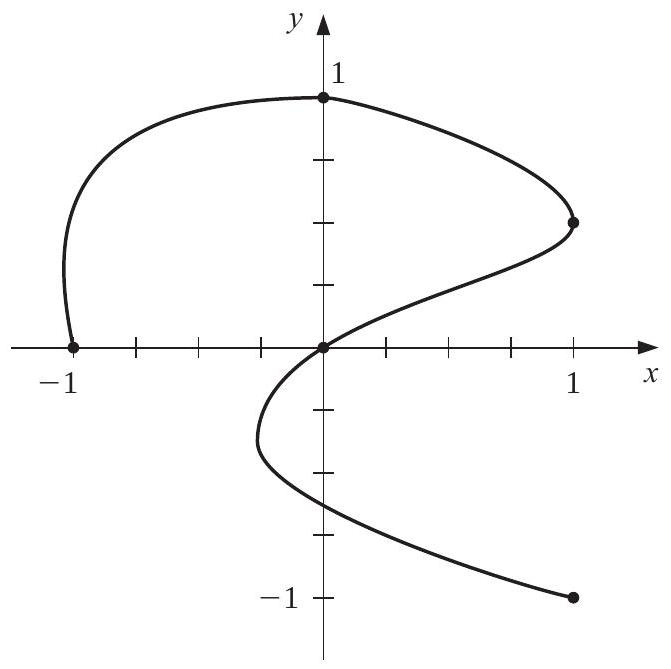
\includegraphics[width=6cm]{2025_05_15_4109a88b43049bd640d1g-61.JPG}
\caption{\scriptsize Figure 1}
\label{fig:2025_05_15_4109a88b43049bd640d1g-61}
\end{figure}

A straightforward parametric technique for determining a polynomial or piecewise polynomial to connect the points $\left(x_{0}, y_{0}\right),\left(x_{1}, y_{1}\right), \ldots,\left(x_{n}, y_{n}\right)$ in the order given is to use a parameter $t$ on an interval $\left[t_{0}, t_{n}\right]$, with $t_{0}<t_{1}<\cdots<t_{n}$, and construct approximation functions with

$$
x_{i}=x\left(t_{i}\right) \quad \text { and } \quad y_{i}=y\left(t_{i}\right), \quad \text { for each } i=0,1, \ldots, n .
$$

The following example demonstrates the technique in the case where both approximating functions are Lagrange interpolating polynomials.

\begin{example}
Construct a pair of Lagrange polynomials to approximate the curve shown in Figure \ref{fig:2025_05_15_4109a88b43049bd640d1g-61}, using the data points shown on the curve.
\end{example}

\begin{mysolution}
There is flexibility in choosing the parameter, and we will choose the points $\left\{t_{i}\right\}_{i=0}^{4}$ equally spaced in $[0,1]$, which gives the data in Table below
\begin{center}
\begin{tabular}{lrlllr}
\hline
$i$ & 0 & 1 & 2 & \multicolumn{1}{c}{3} & 4 \\
\hline
$t_{i}$ & 0 & 0.25 & 0.5 & 0.75 & 1 \\
$x_{i}$ & -1 & 0 & 1 & 0 & 1 \\
$y_{i}$ & 0 & 1 & 0.5 & 0 & -1 \\
\hline
\end{tabular}
\end{center}
This produces the interpolating polynomials
\[x(t)=\left(\left(\left(64 t-\frac{352}{3}\right) t+60\right) t-\frac{14}{3}\right) t-1\]
and
\[y(t)=\left(\left(\left(-\frac{64}{3} t+48\right) t-\frac{116}{3}\right) t+11\right) t.\]
Plotting this parametric system produces the graph shown in blue in Figure \ref{fig:2025_05_15_4109a88b43049bd640d1g-62}. Although it passes through the required points and has the same basic shape, it is quite a crude approximation to the original curve. A more accurate approximation would require additional nodes, with the accompanying increase in computation.
\end{mysolution}

\begin{figure}[h]
\centering
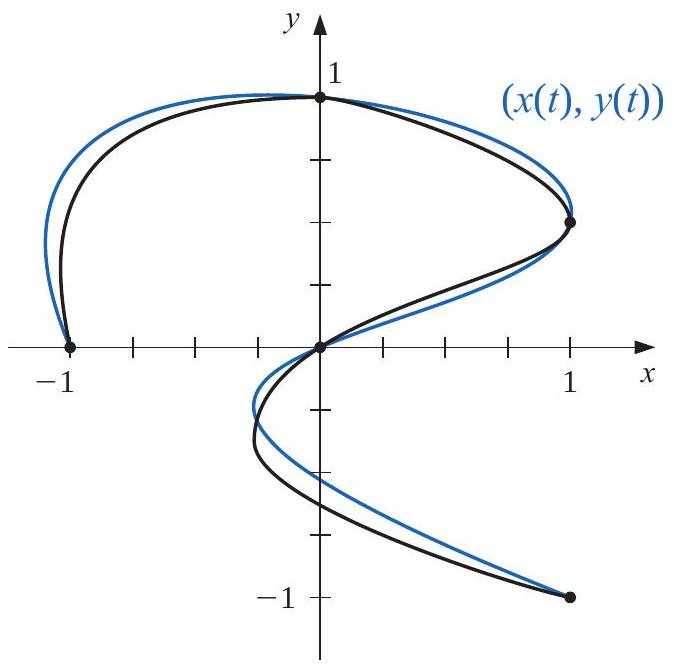
\includegraphics[width=6cm]{2025_05_15_4109a88b43049bd640d1g-62.JPG}
\caption{\scriptsize Figure 2}
\label{fig:2025_05_15_4109a88b43049bd640d1g-62}
\end{figure}


%Figure 3.16
%
%A successful computer design system needs to be based on a formal mathematical theory so that the results are predictable, but this theory should be performed in the background so that the artist can base the design on aesthetics.\\
%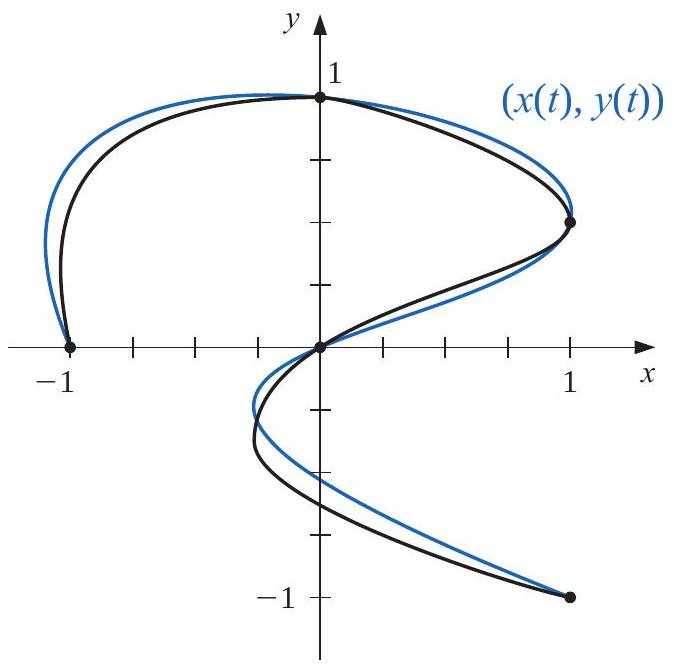
\includegraphics[max width=\textwidth, center]{2025_05_15_4109a88b43049bd640d1g-62}
%
%Parametric Hermite and spline curves can be generated in a similar manner, but these also require extensive computational effort.

%Applications in computer graphics require the rapid generation of smooth curves that can be easily and quickly modified. For both aesthetic and computational reasons, changing one portion of these curves should have little or no effect on other portions of the curves. This eliminates the use of interpolating polynomials and splines since changing one portion of these curves affects the whole curve.
%
The choice of curve for use in computer graphics is generally a form of the piecewise cubic Hermite polynomial. Each portion of a cubic Hermite polynomial is completely determined by specifying its endpoints and the derivatives at these endpoints. As a consequence, one portion of the curve can be changed while leaving most of the curve the same. Only the adjacent portions need to be modified to ensure smoothness at the endpoints. The computations can be performed quickly, and the curve can be modified a section at a time.

The problem with Hermite interpolation is the need to specify the derivatives at the endpoints of each section of the curve. Suppose the curve has $n+1$ data points $\left(x\left(t_{0}\right), y\left(t_{0}\right)\right), \ldots$,\\$\left(x\left(t_{n}\right), y\left(t_{n}\right)\right)$, and we wish to parameterize the cubic to allow complex features. Then we must specify $x^{\prime}\left(t_{i}\right)$ and $y^{\prime}\left(t_{i}\right)$, for each $i=0,1, \ldots, n$. This is not as difficult as it would first appear, since each portion is generated independently. We must ensure only that the derivatives at the endpoints of each portion match those in the adjacent portion. Essentially, then, we can simplify the process to one of determining a pair of cubic Hermite polynomials in the parameter $t$, where $t_{0}=0$ and $t_{1}=1$, given the endpoint data $(x(0), y(0))$ and $(x(1), y(1))$ and the derivatives $d y / d x$ (at $t=0$ ) and $d y / d x$ (at $t=1$ ).

Notice, however, that we are specifying only six conditions, and the cubic polynomials in $x(t)$ and $y(t)$ each have four parameters, for a total of eight. This provides flexibility in choosing the pair of cubic Hermite polynomials to satisfy the conditions, because the natural form for determining $x(t)$ and $y(t)$ requires that we specify $x^{\prime}(0), x^{\prime}(1), y^{\prime}(0)$, and $y^{\prime}(1)$. The explicit Hermite curve in $x$ and $y$ requires specifying only the quotients

$$
\frac{d y}{d x}(t=0)=\frac{y^{\prime}(0)}{x^{\prime}(0)} \quad \text { and } \quad \frac{d y}{d x}(t=1)=\frac{y^{\prime}(1)}{x^{\prime}(1)} .
$$

By multiplying $x^{\prime}(0)$ and $y^{\prime}(0)$ by a common scaling factor, the tangent line to the curve at $(x(0), y(0))$ remains the same, but the shape of the curve varies. The larger the scaling\\
factor, the closer the curve comes to approximating the tangent line near $(x(0), y(0))$. A similar situation exists at the other endpoint $(x(1), y(1))$.

To further simplify the process in interactive computer graphics, the derivative at an endpoint is specified by using a second point, called a guide point, on the desired tangent line. The farther the guide point is from the node, the more closely the curve approximates the tangent line near the node.

In Figure \ref{fig:2025_05_15_4109a88b43049bd640d1g-63(1)}, the nodes occur at ( $x_{0}, y_{0}$ ) and ( $x_{1}, y_{1}$ ), the guide point for ( $x_{0}, y_{0}$ ) is \\$\left(x_{0}+\alpha_{0}, y_{0}+\beta_{0}\right)$, and the guide point for $\left(x_{1}, y_{1}\right)$ is $\left(x_{1}-\alpha_{1}, y_{1}-\beta_{1}\right)$. The cubic Hermite polynomial $x(t)$ on $[0,1]$ satisfies

$$
x(0)=x_{0}, \quad x(1)=x_{1}, \quad x^{\prime}(0)=\alpha_{0}, \quad \text { and } \quad x^{\prime}(1)=\alpha_{1} .
$$

%Figure 3.17\\
\begin{figure}
\centering
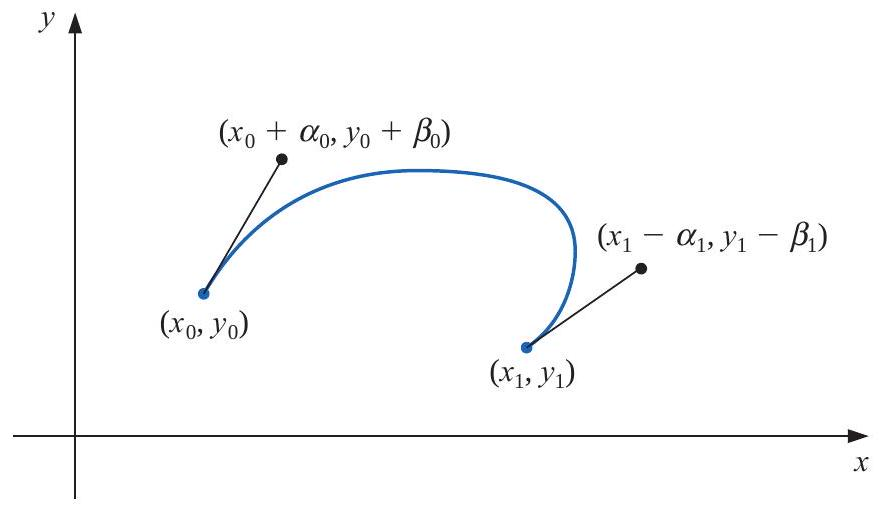
\includegraphics[width=9cm]{2025_05_15_4109a88b43049bd640d1g-63(1).JPG}
\caption{\scriptsize Figure 3 }
\label{fig:2025_05_15_4109a88b43049bd640d1g-63(1)}
\end{figure}

The unique cubic polynomial satisfying these conditions is


\begin{equation}\label{eqn:paramet1}
x(t)=\left[2\left(x_{0}-x_{1}\right)+\left(\alpha_{0}+\alpha_{1}\right)\right] t^{3}+\left[3\left(x_{1}-x_{0}\right)-\left(\alpha_{1}+2 \alpha_{0}\right)\right] t^{2}+\alpha_{0} t+x_{0}
\end{equation}


In a similar manner, the unique cubic polynomial satisfying

$$
y(0)=y_{0}, \quad y(1)=y_{1}, \quad y^{\prime}(0)=\beta_{0}, \quad \text { and } \quad y^{\prime}(1)=\beta_{1}
$$

is


\begin{equation}\label{eqn:paramet2}
y(t)=\left[2\left(y_{0}-y_{1}\right)+\left(\beta_{0}+\beta_{1}\right)\right] t^{3}+\left[3\left(y_{1}-y_{0}\right)-\left(\beta_{1}+2 \beta_{0}\right)\right] t^{2}+\beta_{0} t+y_{0}
\end{equation}


\begin{example}
Determine the graph of the parametric curve generated Eq. \ref{eqn:paramet1} and \ref{eqn:paramet2} when the end points are $\left(x_{0}, y_{0}\right)=(0,0)$ and $\left(x_{1}, y_{1}\right)=(1,0)$, and respective guide points, as shown in Figure \ref{fig:2025_05_15_4109a88b43049bd640d1g-63}
\end{example}

\begin{figure}[h]
\centering
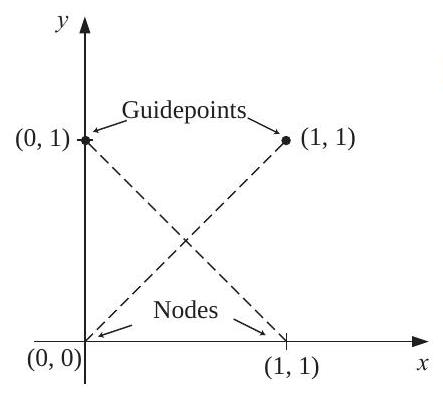
\includegraphics[width=6cm]{2025_05_15_4109a88b43049bd640d1g-63}
\caption{\scriptsize Figure $4$}
\label{fig:2025_05_15_4109a88b43049bd640d1g-63}
\end{figure}
%
%Figure 3.18 Figure 3.18 are $(1,1)$ and $(0,1)$.
%

\begin{mysolution}
The endpoint information implies that $x_{0}=0, x_{1}=1, y_{0}=0$, and $y_{1}=0$, and the guide points at $(1,1)$ and $(0,1)$ imply that $\alpha_{0}=1, \alpha_{1}=1, \beta_{0}=1$, and $\beta_{1}=-1$. Note that the slopes of the guide lines at $(0,0)$ and $(1,0)$ are, respectively

$$
\frac{\beta_{0}}{\alpha_{0}}=\frac{1}{1}=1 \quad \text { and } \quad \frac{\beta_{1}}{\alpha_{1}}=\frac{-1}{1}=-1
$$

Equations \ref{eqn:paramet1} and \ref{eqn:paramet2} imply that for $t \in[0,1]$ we have

$$
x(t)=[2(0-1)+(1+1)] t^{3}+[3(0-0)-(1+2 \cdot 1)] t^{2}+1 \cdot t+0=t
$$

and

$$
y(t)=[2(0-0)+(1+(-1))] t^{3}+[3(0-0)-(-1+2 \cdot 1)] t^{2}+1 \cdot t+0=-t^{2}+t .
$$

This graph is shown as (a) in Figure \ref{fig:2025_05_15_4109a88b43049bd640d1g-64}, together with some other possibilities of curves produced by Eqs. \ref{eqn:paramet1} and \ref{eqn:paramet2} when the nodes are $(0,0)$ and $(1,0)$ and the slopes at these nodes are $1$ and $-1$ , respectively.
\end{mysolution}

\begin{figure}[h]
\centering
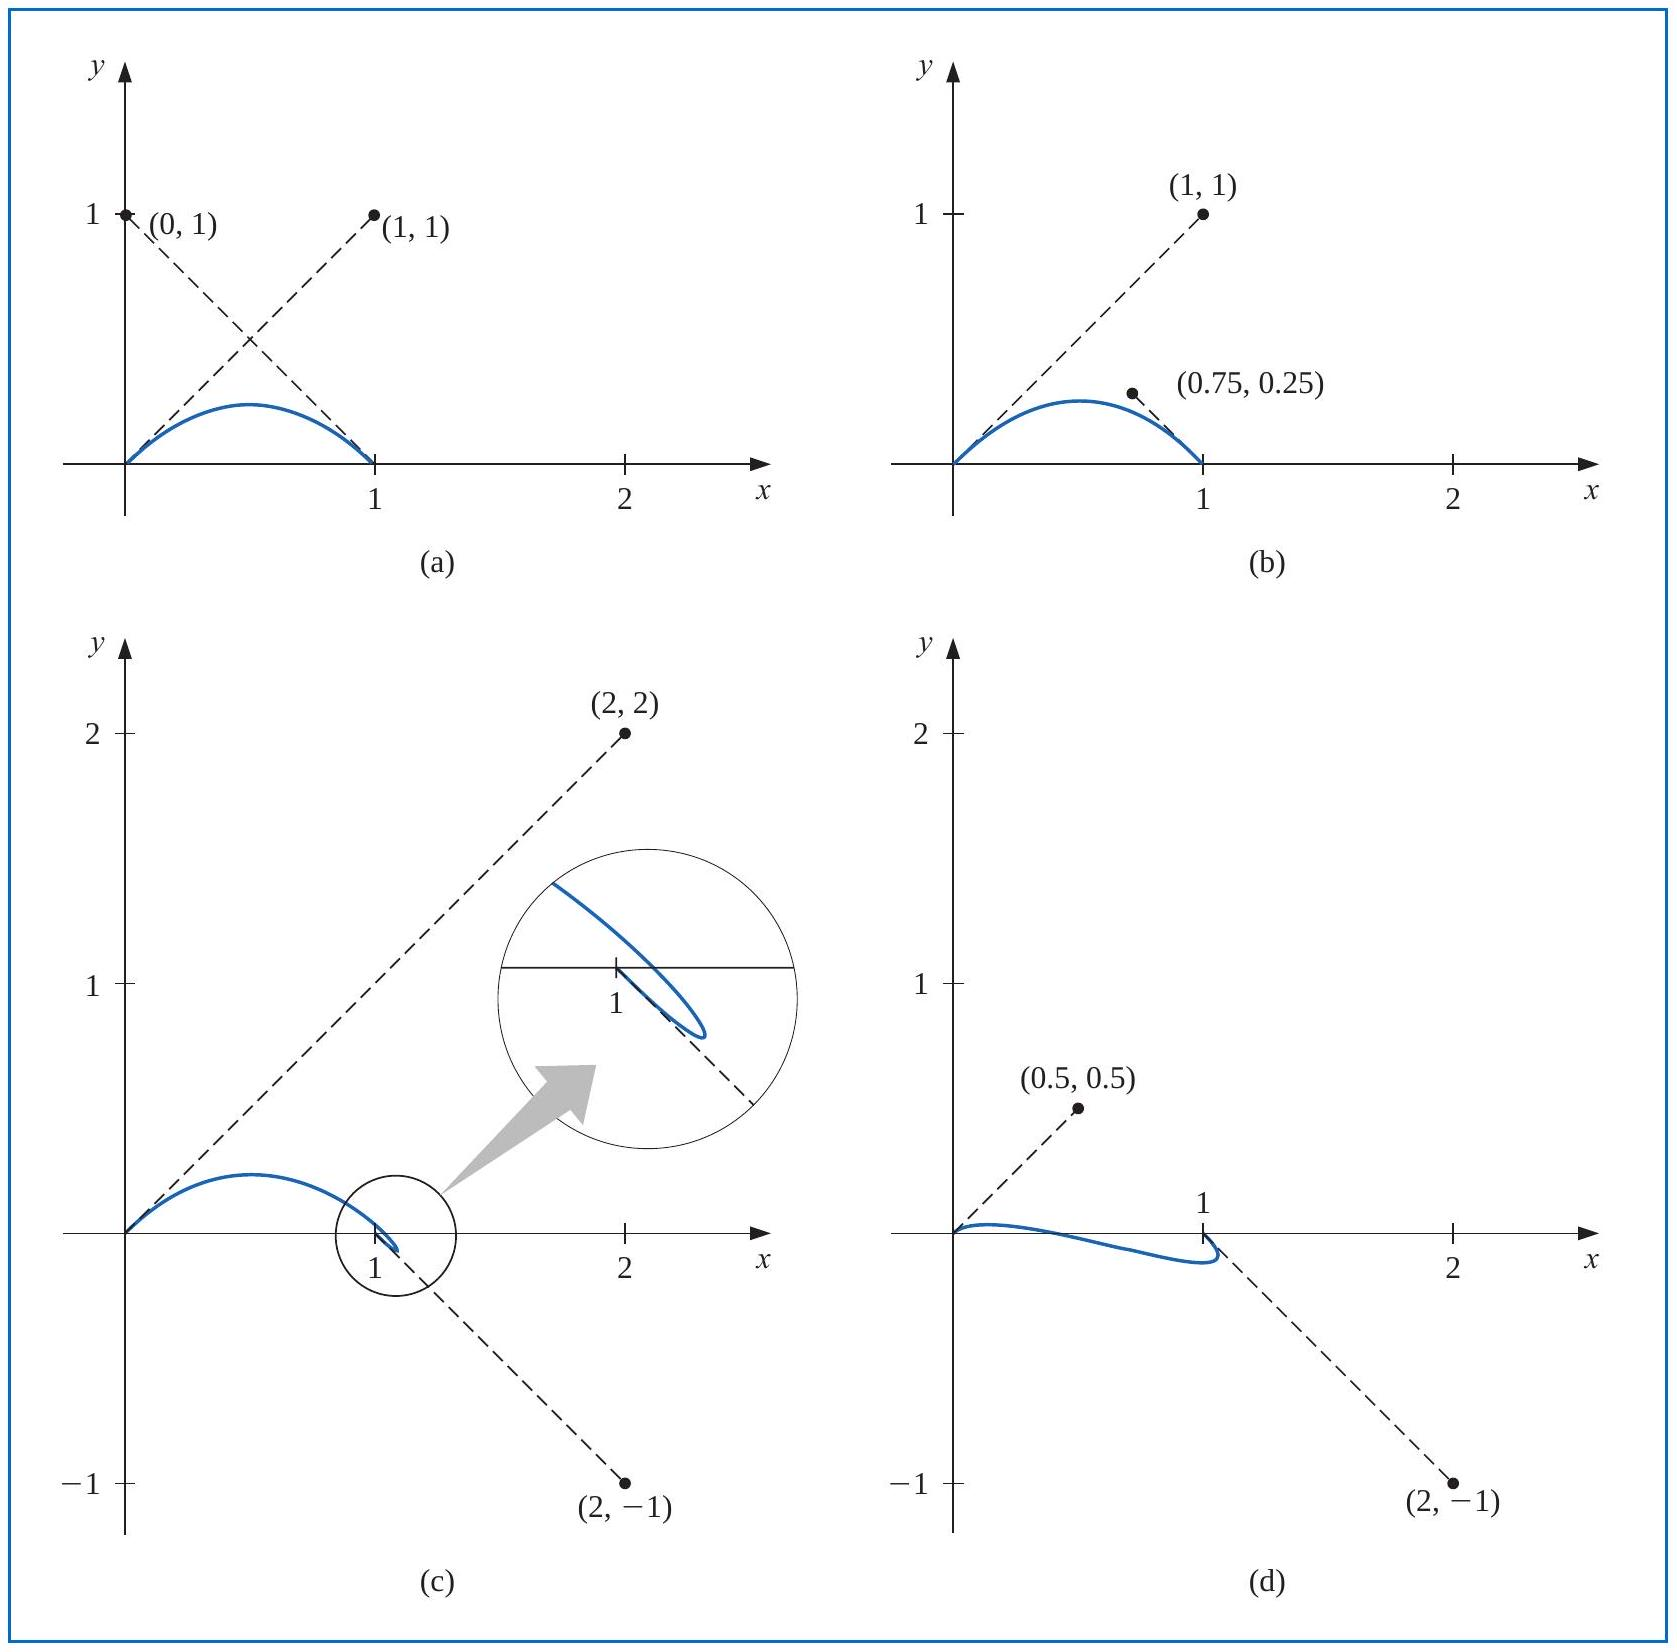
\includegraphics[width=13cm]{2025_05_15_4109a88b43049bd640d1g-64.JPG}
\caption{\scriptsize Figure $5$}
\label{fig:2025_05_15_4109a88b43049bd640d1g-64}
\end{figure}

%Pierre Etienne Bézier (1910-1999) was head of design and production for Renault motorcars for most of his professional life. He began his research into computer-aided design and manufacturing in 1960, developing interactive tools for curve and surface design, and initiated computer-generated milling for automobile modeling.
%
%The Bézier curves that bear his name have the advantage of being based on a rigorous mathematical theory that does not need to be explicitly recognized by the practitioner who simply wants to make an aesthetically pleasing curve or surface. These are the curves that are the basis of the powerful Adobe Postscript system, and produce the freehand curves that are generated in most sufficiently powerful computer graphics packages.\\
%\includegraphics[max width=\textwidth, center]{2025_05_15_4109a88b43049bd640d1g-65}
%
The standard procedure for determining curves in an interactive graphics mode is to first use a mouse or touchpad to set the nodes and guidepoints to generate a first approximation to the curve. These can be set manually, but most graphics systems permit you to use your input device to draw the curve on the screen freehand and will select appropriate nodes and guidepoints for your freehand curve.

The nodes and guidepoints can then be manipulated into a position that produces an aesthetically pleasing curve. Since the computation is minimal, the curve can be determined so quickly that the resulting change is seen immediately. Moreover, all the data needed to compute the curves are imbedded in the coordinates of the nodes and guidepoints, so no analytical knowledge is required of the user.

Popular graphics programs use this type of system for their freehand graphic representations in a slightly modified form. The Hermite cubics are described as {\bf Bézier polynomials}, which incorporate a scaling factor of $3$ when computing the derivatives at the endpoints. This modifies the parametric equations to


\begin{equation}\label{eqn:paramet3}
x(t)=\left[2\left(x_{0}-x_{1}\right)+3\left(\alpha_{0}+\alpha_{1}\right)\right] t^{3}+\left[3\left(x_{1}-x_{0}\right)-3\left(\alpha_{1}+2 \alpha_{0}\right)\right] t^{2}+3 \alpha_{0} t+x_{0}, 
\end{equation}


and


\begin{equation}\label{eqn:paramet4}
y(t)=\left[2\left(y_{0}-y_{1}\right)+3\left(\beta_{0}+\beta_{1}\right)\right] t^{3}+\left[3\left(y_{1}-y_{0}\right)-3\left(\beta_{1}+2 \beta_{0}\right)\right] t^{2}+3 \beta_{0} t+y_{0}, \tag{3.26}
\end{equation}


for $0 \leq t \leq 1$, but this change is transparent to the user of the system.

%Algorithm 3.6 constructs a set of Bézier curves based on the parametric equations in Eqs. (3.25) and (3.26).
%
%\section*{Bézier Curve}
%To construct the cubic Bézier curves $C_{0}, \ldots, C_{n-1}$ in parametric form, where $C_{i}$ is represented by
%
%$$
%\left(x_{i}(t), y_{i}(t)\right)=\left(a_{0}^{(i)}+a_{1}^{(i)} t+a_{2}^{(i)} t^{2}+a_{3}^{(i)} t^{3}, b_{0}^{(i)}+b_{1}^{(i)} t+b_{2}^{(i)} t^{2}+b_{3}^{(i)} t^{3}\right)
%$$
%
%for $0 \leq t \leq 1$, as determined by the left endpoint ( $x_{i}, y_{i}$ ), left guidepoint ( $x_{i}^{+}, y_{i}^{+}$), right endpoint ( $x_{i+1}, y_{i+1}$ ), and right guidepoint ( $x_{i+1}^{-}, y_{i+1}^{-}$) for each $i=0,1, \ldots, n-1$ :\\
%INPUT $n ;\left(x_{0}, y_{0}\right), \ldots,\left(x_{n}, y_{n}\right) ;\left(x_{0}^{+}, y_{0}^{+}\right), \ldots,\left(x_{n-1}^{+}, y_{n-1}^{+}\right) ;\left(x_{1}^{-}, y_{1}^{-}\right), \ldots,\left(x_{n}^{-}, y_{n}^{-}\right)$.\\
%OUTPUT coefficients $\left\{a_{0}^{(i)}, a_{1}^{(i)}, a_{2}^{(i)}, a_{3}^{(i)}, b_{0}^{(i)}, b_{1}^{(i)}, b_{2}^{(i)}, b_{3}^{(i)}\right.$, for $\left.0 \leq i \leq n-1\right\}$.\\
%Step 1 For each $i=0,1, \ldots, n-1$ do Steps 2 and 3 .\\
%Step 2 Set $a_{0}^{(i)}=x_{i}$;
%
%$$
%\begin{aligned}
%b_{0}^{(i)} & =y_{i} ; \\
%a_{1}^{(i)} & =3\left(x_{i}^{+}-x_{i}\right) ; \\
%b_{1}^{(i)} & =3\left(y_{i}^{+}-y_{i}\right) ; \\
%a_{2}^{(i)} & =3\left(x_{i}+x_{i+1}^{-}-2 x_{i}^{+}\right) ; \\
%b_{2}^{(i)} & =3\left(y_{i}+y_{i+1}^{-}-2 y_{i}^{+}\right) ; \\
%a_{3}^{(i)} & =x_{i+1}-x_{i}+3 x_{i}^{+}-3 x_{i+1}^{-} ; \\
%b_{3}^{(i)} & =y_{i+1}-y_{i}+3 y_{i}^{+}-3 y_{i+1}^{-} ;
%\end{aligned}
%$$
%
%Step 3 OUTPUT $\left(a_{0}^{(i)}, a_{1}^{(i)}, a_{2}^{(i)}, a_{3}^{(i)}, b_{0}^{(i)}, b_{1}^{(i)}, b_{2}^{(i)}, b_{3}^{(i)}\right)$.
%
%\section*{Step 4 STOP.}
%Three-dimensional curves are generated in a similar manner by additionally specifying third components $z_{0}$ and $z_{1}$ for the nodes and $z_{0}+\gamma_{0}$ and $z_{1}-\gamma_{1}$ for the guidepoints. The more difficult problem involving the representation of three-dimensional curves concerns the loss of the third dimension when the curve is projected onto a two-dimensional computer screen. Various projection techniques are used, but this topic lies within the realm of computer graphics. For an introduction to this topic and ways that the technique can be modified for surface representations, see one of the many books on computer graphics methods, such as [FVFH].
\begin{myexercise}%\label{Comprehensionquiz2}
Let $\left(x_{0}, y_{0}\right)=(0,0)$ and $\left(x_{1}, y_{1}\right)=(5,2)$ be the endpoints of a curve. Use the given guidepoints to construct parametric cubic Hermite approximations $(x(t), y(t))$ to the curve, and graph the approximations.

\begin{enumerate}[label=(\alph*)]
\item $(1,1)$ and $(6,1)$
\item $(1,1)$ and $(6,3)$
\item $(0.5, 0.5)$ and $(5.5, 1.5)$
\item $(2,2)$ and $(7,0)$
\end{enumerate}
\begin{mysolution}
\begin{enumerate}[label=(\alph*)]
\item $x(t)=-10t^3+14t^2+t$, $y(t)=-2t^3+3t^2+t$
\item $x(t)=-10t^3+14.5t^2+0.5t$, $y(t)=-3t^3+4.5t^2+0.5t$
\item $x(t)=-10t^3+14t^2+t$, $y(t)=-4t^3+5t^2+t$
\item $x(t)=-10t^3+13t^2+2t$, $y(t)=2t$
\end{enumerate}
\end{mysolution}
\end{myexercise}

\section{Numerical Diffrentiation}

\begin{youtube}
This video presents a discussion on numerical differentiation. Follow the discussion and then solve the problems in the subsequent quiz.
\end{youtube}
\mylink{https://www.youtube.com/watch?\\v=-3MwUJCDjts\&list=PLDea8VeK4MUTppAXQzHBNz3KiyEd9SQms\&index=82}

\mylink{https://www.youtube.com/watch?\\v=bKu\_MfpdUiQ\&list=PLDea8VeK4MUTppAXQzHBNz3KiyEd9SQms\&index=83}

\mylink{https://www.youtube.com/watch?\\v=VIXiLXYLjZY\&list=PLDea8VeK4MUTppAXQzHBNz3KiyEd9SQms\&index=84}

\mylink{https://www.youtube.com/watch?\\v=AvvvE3oqHDE\&list=PLDea8VeK4MUTppAXQzHBNz3KiyEd9SQms\&index=86}

\mylink{https://www.youtube.com/watch?v=AVvX-\\DyV3wQ\&list=PLDea8VeK4MUTppAXQzHBNz3KiyEd9SQms\&index=87}

\mylink{https://www.youtube.com/watch?\\v=RJhbUvyTBf0\&list=PLDea8VeK4MUTppAXQzHBNz3KiyEd9SQms\&index=88}

\mylink{https://www.youtube.com/watch?\\v=L\_80gD1TJSI\&list=PLDea8VeK4MUTppAXQzHBNz3KiyEd9SQms\&index=89}

Consider the following example

\begin{example} \label{numediffexample1}
Use the forward-difference formula to approximate the derivative of $f(x)=\ln x$ at $x_{0}=1.8$ using $h=0.1, h=0.05$, and $h=0.01$, and determine bounds for the approximation errors.
\end{example}
\begin{mysolution} 
The forward-difference formula

$$
\frac{f(1.8+h)-f(1.8)}{h}
$$

with $h=0.1$ gives

$$
\frac{\ln 1.9-\ln 1.8}{0.1}=\frac{0.64185389-0.58778667}{0.1}=0.5406722
$$

Because $f^{\prime \prime}(x)=-1 / x^{2}$ and $1.8<\xi<1.9$, a bound for this approximation error is

$$
\frac{\left|h f^{\prime \prime}(\xi)\right|}{2}=\frac{|h|}{2 \xi^{2}}<\frac{0.1}{2(1.8)^{2}}=0.0154321
$$

The approximation and error bounds when $h=0.05$ and $h=0.01$ are found in a similar manner and the results are shown in Table \ref{table1}.

%Table 4.1



Since $f^{\prime}(x)=1 / x$, the exact value of $f^{\prime}(1.8)$ is $0.55 \overline{5}$, and in this case the error bounds are quite close to the true approximation error.\qed
\end{mysolution}

\begin{figure}
\centering
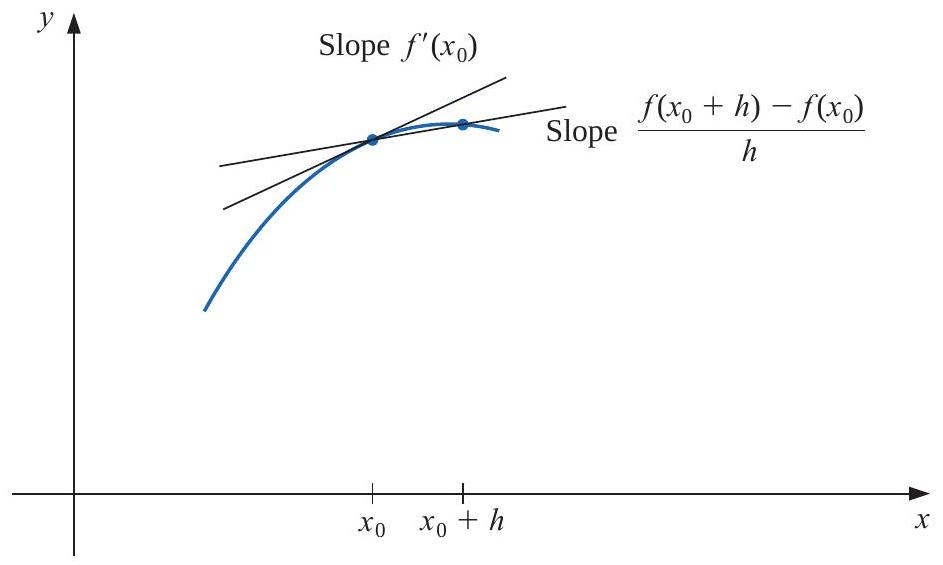
\includegraphics[width=10cm]{2025_05_15_85b7f7df47271a498e1dg-03}
\caption{\scriptsize Figure $6$}
\label{figure6}
\end{figure}

\begin{table}[h]
\centering
\begin{tabular}{lccc}
\hline
\multicolumn{1}{c}{$h$} & $f(1.8+h)$ & $\frac{f(1.8+h)-f(1.8)}{h}$ & $\frac{|h|}{2(1.8)^{2}}$ \\
\hline
0.1 & 0.64185389 & 0.5406722 & 0.0154321 \\
0.05 & 0.61518564 & 0.5479795 & 0.0077160 \\
0.01 & 0.59332685 & 0.5540180 & 0.0015432 \\
\hline
\end{tabular}
\caption{\scriptsize Table $1$}
\label{table1}
\end{table}

\begin{myexercise}%\label{Comprehensionquiz2}
Use the forward-difference formulas and backward-difference formulas to determine each missing entry in the following tables.
\begin{multicols}{2}
\begin{enumerate}[label=(\alph*)]
\item
\begin{center}
\begin{tabular}{c|c|l}
$x$ & $f(x)$ & $f^{\prime}(x)$ \\
\hline
0.5 & 0.4794 &  \\
0.6 & 0.5646 &  \\
0.7 & 0.6442 &  \\
\end{tabular}
\end{center}
\item
\begin{center}
\begin{tabular}{c|l|l}
$x$ & \multicolumn{1}{|c|}{$f(x)$} & $f^{\prime}(x)$ \\
\hline
0.0 & 0.00000 &  \\
0.2 & 0.74140 &  \\
0.4 & 1.3718 &  \\
\end{tabular}
\end{center}
\end{enumerate}
\end{multicols}
\begin{mysolution}
From the forward-backward difference formula we have the following approximations:
 \begin{enumerate}[label=(\alph*)]
\item $f'(0.5)\approx0.8520$, $f(0.6)\approx0.8520$, $f(0.7)\approx0.7960$
\item $f'(0.0)\approx3.7070$, $f(0.2)\approx3.1520$, $f(0.4\approx3.1520$
\end{enumerate}
\end{mysolution}
\end{myexercise}



\section{Richardson's Extrapolation}
\activities
Read on Richardson's extrapolation in the reference provided in the link below in the pages Appendix C1 and then attempt the subsequent quiz.
\begin{activity}[\cg Reading]
%\begin{enumerate}
%\item \mylink{https://math.libretexts.org/Bookshelves/Calculus/CLP-2\_Integral\_Calculus\_(Feldman\_Rechnitzer\_and\_Yeager)/04\%3A\_Appendices/4.03\%3A\_C\%3A\_More\_About\_Numerical\_Integration/4.3.01\%3A\_C.1\%3A\_Richardson\_Extrapolation}
%\end{enumerate}
\mylink{https://math.libretexts.org/Bookshelves/Calculus/\\CLP-2\_Integral\_Calculus\_(Feldman\_Rechnitzer\_and\_Yeager)}
\end{activity}

\begin{example}\label{Richardsonsexample1}
In Example \ref{numediffexample1} of Section 2 we use the forward-difference method with $h=0.1$ and $h=0.05$ to find approximations to $f^{\prime}(1.8)$ for $f(x)=\ln (x)$. Assume that this formula has truncation error $O(h)$ and use extrapolation on these values to see if this results in a better approximation.
\end{example}

\begin{mysolution}
In Example \ref{numediffexample1} of Section 2 we found that

$$
\text { with } h=0.1: f^{\prime}(1.8) \approx 0.5406722, \quad \text { and } \quad \text { with } h=0.05: f^{\prime}(1.8) \approx 0.5479795 .
$$

This implies that

$$
N_{1}(0.1)=0.5406722 \text { and } N_{1}(0.05)=0.5479795 .
$$

Extrapolating these results gives the new approximation

$$
\begin{aligned}
N_{2}(0.1) & =N_{1}(0.05)+\left(N_{1}(0.05)-N_{1}(0.1)\right)=0.5479795+(0.5479795-0.5406722) \\
& =0.555287
\end{aligned}
$$

The $h=0.1$ and $h=0.05$ results were found to be accurate to within $1.5 \times 10^{-2}$ and $7.7 \times 10^{-3}$, respectively. Because $f^{\prime}(1.8)=1 / 1.8=0 . \overline{5}$, the extrapolated value is accurate to within $2.7 \times 10^{-4}$.
\end{mysolution}
\begin{myexercise}%\label{Comprehensionquiz2}
Apply the extrapolation process described in Example \ref{Richardsonsexample1} to determine $N_{3}(h)$, an approximation to $f^{\prime}\left(x_{0}\right)$, for the following functions and stepsizes.
%%\begin{multicols}{2}
\begin{enumerate}[label=(\alph*)]
\item $\quad f(x)=\ln x, x_{0}=1.0, h=0.4$\\
\item $\quad f(x)=x+e^{x}, x_{0}=0.0, h=0.4$\\
\item $\quad f(x)=2^{x} \sin x, x_{0}=1.05, h=0.4$\\
\item $\quad f(x)=x^{3} \cos x, x_{0}=2.3, h=0.4$
\end{enumerate}
%\end{multicols}

\begin{mysolution}
\begin{multicols}{2}
\begin{enumerate}[label=(\alph*)]
\item $f(1)\approx1.0000109$ \item $f(0)\approx2.0000000$ \item $f(1.05)\approx2.2751459$ \item $f(2.3)\approx-19.646799$
\end{enumerate}
\end{multicols}
\end{mysolution}
\end{myexercise}


\section{Elements of Numerical Integration}
%\begin{youtube}
%This video presents a discussion on elements of numerical integration. Follow the discussion and then solve the problems in the subsequent quiz.
%\end{youtube}

\videolesson
\begin{selfvideo}[2]
%LESSON 3: 
This video presents a discussion on elements of numerical integration. Follow the discussion and then solve the problems in the subsequent quiz.
\end{selfvideo}

%\mylink{https://www.youtube.com/watch?v=2ypA51D945g\&list=PLDea8VeK4MUTppAXQzHBNz3KiyEd9SQms\&index=91}
%
%\mylink{https://www.youtube.com/watch?v=cE1WjwLTXMI\&list=PLDea8VeK4MUTppAXQzHBNz3KiyEd9SQms\&index=92}
%
%\mylink{https://www.youtube.com/watch?v=z8C1lXfsAC0\&list=PLDea8VeK4MUTppAXQzHBNz3KiyEd9SQms\&index=93}
%\begin{boxB}Question: \end{boxB}


The need often arises for evaluating the definite integral of a function that has no explicit antiderivative or whose antiderivative is not easy to obtain. The basic method involved in approximating $\int_{a}^{b} f(x) d x$ is called numerical quadrature. It uses a sum $\sum_{i=0}^{n} a_{i} f\left(x_{i}\right)$ to approximate $\int_{a}^{b} f(x) d x$.

The methods of quadrature in this section are based on the interpolation polynomials given in Chapter 3. The basic idea is to select a set of distinct nodes $\left\{x_{0}, \ldots, x_{n}\right\}$ from the interval $[a, b]$. Then integrate the Lagrange interpolating polynomial

$$
P_{n}(x)=\sum_{i=0}^{n} f\left(x_{i}\right) L_{i}(x)
$$

and its truncation error term over $[a, b]$ to obtain

$$
\begin{aligned}
\int_{a}^{b} f(x) d x & =\int_{a}^{b} \sum_{i=0}^{n} f\left(x_{i}\right) L_{i}(x) d x+\int_{a}^{b} \prod_{i=0}^{n}\left(x-x_{i}\right) \frac{f^{(n+1)}(\xi(x))}{(n+1)!} d x \\
& =\sum_{i=0}^{n} a_{i} f\left(x_{i}\right)+\frac{1}{(n+1)!} \int_{a}^{b} \prod_{i=0}^{n}\left(x-x_{i}\right) f^{(n+1)}(\xi(x)) d x
\end{aligned}
$$

where $\xi(x)$ is in $[a, b]$ for each $x$ and

$$
a_{i}=\int_{a}^{b} L_{i}(x) d x, \quad \text { for each } i=0,1, \ldots, n
$$

The quadrature formula is, therefore,

$$
\int_{a}^{b} f(x) d x \approx \sum_{i=0}^{n} a_{i} f\left(x_{i}\right)
$$

with error given by

$$
E(f)=\frac{1}{(n+1)!} \int_{a}^{b} \prod_{i=0}^{n}\left(x-x_{i}\right) f^{(n+1)}(\xi(x)) d x
$$

Before discussing the general situation of quadrature formulas, let us consider formulas produced by using first and second Lagrange polynomials with equally-spaced nodes. This gives the {\bf Trapezoidal rule} and {\bf Simpson's rule}, which are commonly introduced in calculus courses.

When we use the term trapezoid we mean a four-sided figure that has at least two of its sides parallel. The European term for this figure is trapezium. To further confuse the issue, the European word trapezoidal refers to a four-sided figure with no sides equal, and the American word for this type of figure is trapezium.

\subsection*{The Trapezoidal Rule}
To derive the Trapezoidal rule for approximating $\int_{a}^{b} f(x) d x$, let $x_{0}=a, x_{1}=b, h=b-a$ and use the linear Lagrange polynomial:

$$
P_{1}(x)=\frac{\left(x-x_{1}\right)}{\left(x_{0}-x_{1}\right)} f\left(x_{0}\right)+\frac{\left(x-x_{0}\right)}{\left(x_{1}-x_{0}\right)} f\left(x_{1}\right)
$$

Then


\begin{equation}\label{eqn:traprule1}
\begin{split}
\int_{a}^{b} f(x) d x= & \int_{x_{0}}^{x_{1}}\left[\frac{\left(x-x_{1}\right)}{\left(x_{0}-x_{1}\right)} f\left(x_{0}\right)+\frac{\left(x-x_{0}\right)}{\left(x_{1}-x_{0}\right)} f\left(x_{1}\right)\right] d x \\
& +\frac{1}{2} \int_{x_{0}}^{x_{1}} f^{\prime \prime}(\xi(x))\left(x-x_{0}\right)\left(x-x_{1}\right) d x 
\end{split}
\end{equation}


The product $\left(x-x_{0}\right)\left(x-x_{1}\right)$ does not change sign on $\left[x_{0}, x_{1}\right]$, so the Weighted Mean Value Theorem for Integrals 1.13 can be applied to the error term to give, for some $\xi$ in ( $x_{0}, x_{1}$ ),

$$
\begin{aligned}
\int_{x_{0}}^{x_{1}} f^{\prime \prime}(\xi(x))\left(x-x_{0}\right)\left(x-x_{1}\right) d x & =f^{\prime \prime}(\xi) \int_{x_{0}}^{x_{1}}\left(x-x_{0}\right)\left(x-x_{1}\right) d x \\
& =f^{\prime \prime}(\xi)\left[\frac{x^{3}}{3}-\frac{\left(x_{1}+x_{0}\right)}{2} x^{2}+x_{0} x_{1} x\right]_{x_{0}}^{x_{1}} \\
& =-\frac{h^{3}}{6} f^{\prime \prime}(\xi)
\end{aligned}
$$

Consequently, Eq. \ref{eqn:traprule1} implies that

$$
\begin{aligned}
\int_{a}^{b} f(x) d x & =\left[\frac{\left(x-x_{1}\right)^{2}}{2\left(x_{0}-x_{1}\right)} f\left(x_{0}\right)+\frac{\left(x-x_{0}\right)^{2}}{2\left(x_{1}-x_{0}\right)} f\left(x_{1}\right)\right]_{x_{0}}^{x_{1}}-\frac{h^{3}}{12} f^{\prime \prime}(\xi) \\
& =\frac{\left(x_{1}-x_{0}\right)}{2}\left[f\left(x_{0}\right)+f\left(x_{1}\right)\right]-\frac{h^{3}}{12} f^{\prime \prime}(\xi)
\end{aligned}
$$

Using the notation $h=x_{1}-x_{0}$ gives the following rule:\\

\begin{boxB}{\bf Trapezoidal Rule:}
$$
\int_{a}^{b} f(x) d x=\frac{h}{2}\left[f\left(x_{0}\right)+f\left(x_{1}\right)\right]-\frac{h^{3}}{12} f^{\prime \prime}(\xi)
$$
 \end{boxB}

This is called the Trapezoidal rule because when $f$ is a function with positive values, $\int_{a}^{b} f(x) d x$ is approximated by the area in a trapezoid, as shown in Figure \ref{fig:trapezoid1}.

%Figure 4.3\\
\begin{figure}[h]
\centering
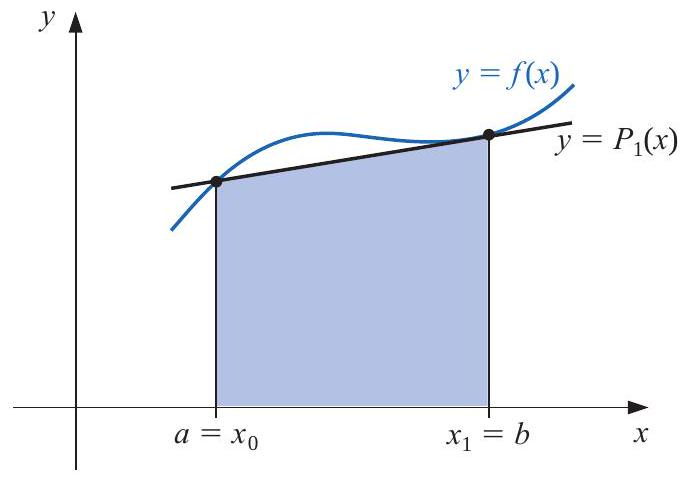
\includegraphics[width=10cm]{2025_05_15_85b7f7df47271a498e1dg-22}
\caption{\scriptsize Figure $7$}
\label{fig:trapezoid1}
\end{figure}

The error term for the Trapezoidal rule involves $f^{\prime \prime}$, so the rule gives the exact result when applied to any function whose second derivative is identically zero, that is, any polynomial of degree one or less.

\subsection*{Simpson's Rule}
Simpson's rule results from integrating over $[a, b]$ the second Lagrange polynomial with equally-spaced nodes $x_{0}=a, x_{2}=b$, and $x_{1}=a+h$, where $h=(b-a) / 2$. (See Figure \ref{fig:simpfig1}.)

%Figure 4.4\\
\begin{figure}[h]
\centering
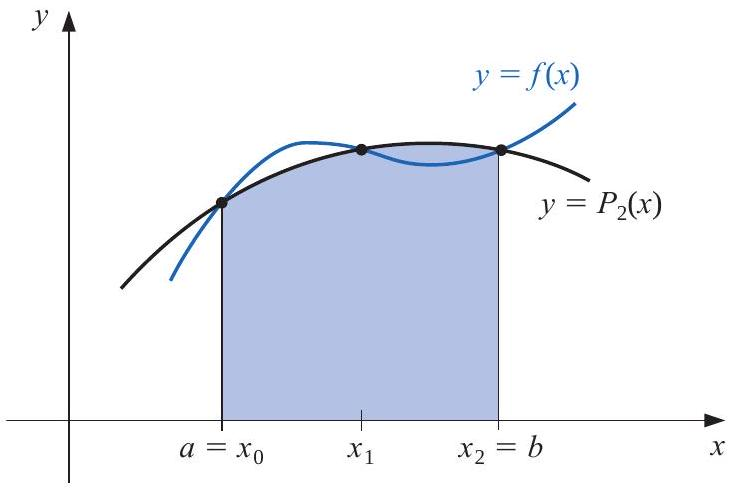
\includegraphics[width=10cm]{2025_05_15_85b7f7df47271a498e1dg-23}
\caption{\scriptsize Figure $8$}
\label{fig:simpfig1}
\end{figure}

Therefore

$$
\begin{aligned}
\int_{a}^{b} f(x) d x= & \int_{x_{0}}^{x_{2}}\left[\frac{\left(x-x_{1}\right)\left(x-x_{2}\right)}{\left(x_{0}-x_{1}\right)\left(x_{0}-x_{2}\right)} f\left(x_{0}\right)+\frac{\left(x-x_{0}\right)\left(x-x_{2}\right)}{\left(x_{1}-x_{0}\right)\left(x_{1}-x_{2}\right)} f\left(x_{1}\right)\right. \\
& \left.+\frac{\left(x-x_{0}\right)\left(x-x_{1}\right)}{\left(x_{2}-x_{0}\right)\left(x_{2}-x_{1}\right)} f\left(x_{2}\right)\right] d x \\
& +\int_{x_{0}}^{x_{2}} \frac{\left(x-x_{0}\right)\left(x-x_{1}\right)\left(x-x_{2}\right)}{6} f^{(3)}(\xi(x)) d x
\end{aligned}
$$

Deriving Simpson's rule in this manner, however, provides only an $O\left(h^{4}\right)$ error term involving $f^{(3)}$. By approaching the problem in another way, a higher-order term involving $f^{(4)}$ can be derived.

To illustrate this alternative method, suppose that $f$ is expanded in the third Taylor polynomial about $x_{1}$. Then for each $x$ in $\left[x_{0}, x_{2}\right]$, a number $\xi(x)$ in ( $x_{0}, x_{2}$ ) exists with\\
$f(x)=f\left(x_{1}\right)+f^{\prime}\left(x_{1}\right)\left(x-x_{1}\right)+\frac{f^{\prime \prime}\left(x_{1}\right)}{2}\left(x-x_{1}\right)^{2}+\frac{f^{\prime \prime \prime}\left(x_{1}\right)}{6}\left(x-x_{1}\right)^{3}+\frac{f^{(4)}(\xi(x))}{24}\left(x-x_{1}\right)^{4}$\\
and


\begin{equation}\label{eqn:simpson1}
\begin{split}
\int_{x_{0}}^{x_{2}} f(x) d x= & {\left[f\left(x_{1}\right)\left(x-x_{1}\right)+\frac{f^{\prime}\left(x_{1}\right)}{2}\left(x-x_{1}\right)^{2}+\frac{f^{\prime \prime}\left(x_{1}\right)}{6}\left(x-x_{1}\right)^{3}\right.} \\
& \left.+\frac{f^{\prime \prime \prime}\left(x_{1}\right)}{24}\left(x-x_{1}\right)^{4}\right]_{x_{0}}^{x_{2}}+\frac{1}{24} \int_{x_{0}}^{x_{2}} f^{(4)}(\xi(x))\left(x-x_{1}\right)^{4} d x 
\end{split}
\end{equation}


%Thomas Simpson (1710-1761) was a self-taught mathematician who supported himself during his early years as a weaver. His primary interest was probability theory, although in 1750 he published a two-volume calculus book entitled The Doctrine and Application of Fluxions.

Because $\left(x-x_{1}\right)^{4}$ is never negative on $\left[x_{0}, x_{2}\right]$, the Weighted Mean Value Theorem for Integrals 1.13 implies that

$$
\left.\frac{1}{24} \int_{x_{0}}^{x_{2}} f^{(4)}(\xi(x))\left(x-x_{1}\right)^{4} d x=\frac{f^{(4)}\left(\xi_{1}\right)}{24} \int_{x_{0}}^{x_{2}}\left(x-x_{1}\right)^{4} d x=\frac{f^{(4)}\left(\xi_{1}\right)}{120}\left(x-x_{1}\right)^{5}\right]_{x_{0}}^{x_{2}}
$$

for some number $\xi_{1}$ in ( $x_{0}, x_{2}$ ).\\
However, $h=x_{2}-x_{1}=x_{1}-x_{0}$, so

$$
\left(x_{2}-x_{1}\right)^{2}-\left(x_{0}-x_{1}\right)^{2}=\left(x_{2}-x_{1}\right)^{4}-\left(x_{0}-x_{1}\right)^{4}=0
$$

whereas

$$
\left(x_{2}-x_{1}\right)^{3}-\left(x_{0}-x_{1}\right)^{3}=2 h^{3} \quad \text { and } \quad\left(x_{2}-x_{1}\right)^{5}-\left(x_{0}-x_{1}\right)^{5}=2 h^{5} .
$$

Consequently, Eq. \ref{eqn:simpson1} can be rewritten as

$$
\int_{x_{0}}^{x_{2}} f(x) d x=2 h f\left(x_{1}\right)+\frac{h^{3}}{3} f^{\prime \prime}\left(x_{1}\right)+\frac{f^{(4)}\left(\xi_{1}\right)}{60} h^{5}
$$

If we now replace $f^{\prime \prime}\left(x_{1}\right)$ by the approximation given in Eq. (4.9) of Section 4.1, we have

$$
\begin{aligned}
\int_{x_{0}}^{x_{2}} f(x) d x & =2 h f\left(x_{1}\right)+\frac{h^{3}}{3}\left\{\frac{1}{h^{2}}\left[f\left(x_{0}\right)-2 f\left(x_{1}\right)+f\left(x_{2}\right)\right]-\frac{h^{2}}{12} f^{(4)}\left(\xi_{2}\right)\right\}+\frac{f^{(4)}\left(\xi_{1}\right)}{60} h^{5} \\
& =\frac{h}{3}\left[f\left(x_{0}\right)+4 f\left(x_{1}\right)+f\left(x_{2}\right)\right]-\frac{h^{5}}{12}\left[\frac{1}{3} f^{(4)}\left(\xi_{2}\right)-\frac{1}{5} f^{(4)}\left(\xi_{1}\right)\right]
\end{aligned}
$$

It can be shown by alternative methods that the values $\xi_{1}$ and $\xi_{2}$ in this expression can be replaced by a common value $\xi$ in ( $x_{0}, x_{2}$ ). This gives Simpson's rule.
\begin{boxB}
{\bf Simpson's Rule:}
$$
\int_{x_{0}}^{x_{2}} f(x) d x=\frac{h}{3}\left[f\left(x_{0}\right)+4 f\left(x_{1}\right)+f\left(x_{2}\right)\right]-\frac{h^{5}}{90} f^{(4)}(\xi)
$$
\end{boxB}

The error term in Simpson's rule involves the fourth derivative of $f$, so it gives exact results when applied to any polynomial of degree three or less.

\begin{example}
Compare the Trapezoidal rule and Simpson's rule approximations to $\int_{0}^{2} f(x) d x$ when $f(x)$ is\\
\begin{enumerate}[label=(\alph*)]
\begin{multicols}{3}
\item $x^{2}$
\item $x^{4}$
\item $(x+1)^{-1}$
\item $\sqrt{1+x^{2}}$
\item $\sin x$
\item $e^{x}$
\end{multicols}
\end{enumerate}
\end{example}
\begin{mysolution}
On [0,2] the Trapezoidal and Simpson's rule have the forms\\
Trapezoid: $\int_{0}^{2} f(x) d x \approx f(0)+f(2)$ and Simpson's: $\int_{0}^{2} f(x) d x \approx \frac{1}{3}[f(0)+4 f(1)+f(2)]$.

When $f(x)=x^{2}$ they give

$$
\begin{gathered}
\text { Trapezoid: } \int_{0}^{2} f(x) d x \approx 0^{2}+2^{2}=4 \text { and } \\
\text { Simpson's: } \int_{0}^{2} f(x) d x \approx \frac{1}{3}\left[\left(0^{2}\right)+4 \cdot 1^{2}+2^{2}\right]=\frac{8}{3}
\end{gathered}
$$

The approximation from Simpson's rule is exact because its truncation error involves $f^{(4)}$, which is identically 0 when $f(x)=x^{2}$.

The results to three places for the functions are summarized in Table \ref{tab:simpsonexample1}. Notice that in each instance Simpson's Rule is significantly superior.
\end{mysolution}
%Table 4.7

\begin{table}[h]
\centering
\begin{tabular}{|l|l|l|l|l|l|l|}
\hline
 & (a) & (b) & (c) & (d) & (e) & (f) \\
\hline
$f(x)$ & $x^{2}$ & $x^{4}$ & $(x+1)^{-1}$ & $\sqrt{1+x^{2}}$ & $\sin x$ & $e^{x}$ \\
\hline
Exact value & 2.667 & 6.400 & 1.099 & 2.958 & 1.416 & 6.389 \\
\hline
Trapezoidal & 4.000 & 16.000 & 1.333 & 3.326 & 0.909 & 8.389 \\
\hline
Simpson's & 2.667 & 6.667 & 1.111 & 2.964 & 1.425 & 6.421 \\
\hline
\end{tabular}
\caption{\scriptsize Table 2: Comparison of Trapezoid and Simpson's Rules }
\label{tab:simpsonexample1}
\end{table}


\subsection*{Measuring Precision}
The standard derivation of quadrature error formulas is based on determining the class of polynomials for which these formulas produce exact results. The next definition is used to facilitate the discussion of this derivation.

\begin{definition}\label{def:precision}
The degree of accuracy, or precision, of a quadrature formula is the largest positive integer $n$ such that the formula is exact for $x^{k}$, for each $k=0,1, \ldots, n$.
\end{definition}
%The improved accuracy of Simpson's rule over the Trapezoidal rule is intuitively explained by the fact that Simpson's rule includes a midpoint evaluation that provides better balance to the approximation.
%
%The open and closed terminology for methods implies that the open methods use as nodes only points in the open interval, ( $a, b$ ) to approximate $\int_{a}^{b} f(x) d x$. The closed methods include the points $a$ and $b$ of the closed interval $[a, b]$ as nodes.

Definition \ref{def:precision} implies that the Trapezoidal and Simpson's rules have degrees of precision one and three, respectively.

Integration and summation are linear operations; that is,

$$
\int_{a}^{b}(\alpha f(x)+\beta g(x)) d x=\alpha \int_{a}^{b} f(x) d x+\beta \int_{a}^{b} g(x) d x
$$

and

$$
\sum_{i=0}^{n}\left(\alpha f\left(x_{i}\right)+\beta g\left(x_{i}\right)\right)=\alpha \sum_{i=0}^{n} f\left(x_{i}\right)+\beta \sum_{i=0}^{n} g\left(x_{i}\right),
$$

for each pair of integrable functions $f$ and $g$ and each pair of real constants $\alpha$ and $\beta$. This implies that:

\begin{boxB}
The degree of precision of a quadrature formula is $n$ if and only if the error is zero for all polynomials of degree $k=0,1, \ldots, n$, but is not zero for some polynomial of degree $n+1$.
\end{boxB}

The Trapezoidal and Simpson's rules are examples of a class of methods known as NewtonCotes formulas. There are two types of Newton-Cotes formulas, open and closed.

\subsection*{Closed Newton-Cotes Formulas}
The ( $n+1$ )-point closed Newton-Cotes formula uses nodes $x_{i}=x_{0}+i h$, for $i=0,1, \ldots, n$, where $x_{0}=a, x_{n}=b$ and $h=(b-a) / n$. (See Figure \ref{fig:closednewtoncotes1}.) It is called closed because the endpoints of the closed interval $[a, b]$ are included as nodes.

%Figure 4.5\\
\begin{figure}[h]
\centering
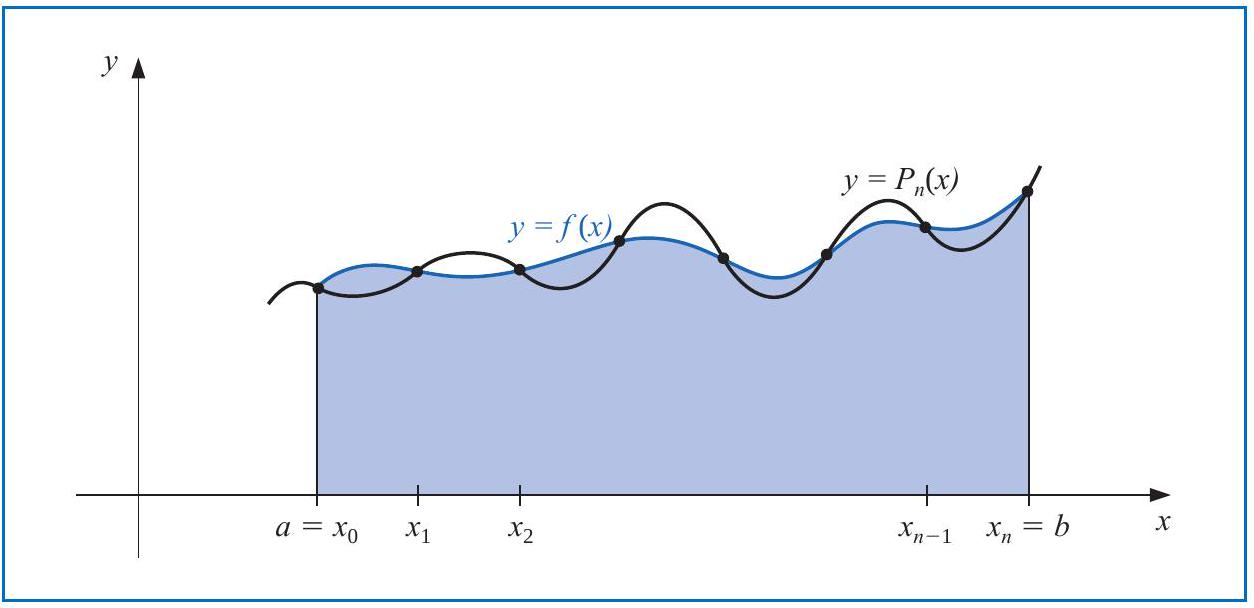
\includegraphics[width=12cm]{2025_05_15_85b7f7df47271a498e1dg-26}
\caption{\scriptsize Figure $9$}
\label{fig:closednewtoncotes1}
\end{figure}
The formula assumes the form

$$
\int_{a}^{b} f(x) d x \approx \sum_{i=0}^{n} a_{i} f\left(x_{i}\right)
$$

where

$$
a_{i}=\int_{x_{0}}^{x_{n}} L_{i}(x) d x=\int_{x_{0}}^{x_{n}} \prod_{\substack{j=0 \\ j \neq i}}^{n} \frac{\left(x-x_{j}\right)}{\left(x_{i}-x_{j}\right)} d x
$$

The following theorem details the error analysis associated with the closed Newton Cotes formulas.

\begin{theorem}\label{thm:closednewtonecotes}
Suppose that $\sum_{i=0}^{n} a_{i} f\left(x_{i}\right)$ denotes the ( $n+1$ )-point closed Newton-Cotes formula with $x_{0}=a, x_{n}=b$, and $h=(b-a) / n$. There exists $\xi \in(a, b)$ for which

%Roger Cotes (1682-1716) rose from a modest background to become, in 1704, the first Plumian Professor at Cambridge University. He made advances in numerous mathematical areas including numerical methods for interpolation and integration.\\
%Newton is reputed to have said of Cotes ...if he had lived we might have known something.

$$
\int_{a}^{b} f(x) d x=\sum_{i=0}^{n} a_{i} f\left(x_{i}\right)+\frac{h^{n+3} f^{(n+2)}(\xi)}{(n+2)!} \int_{0}^{n} t^{2}(t-1) \cdots(t-n) d t
$$

if $n$ is even and $f \in C^{n+2}[a, b]$, and

$$
\int_{a}^{b} f(x) d x=\sum_{i=0}^{n} a_{i} f\left(x_{i}\right)+\frac{h^{n+2} f^{(n+1)}(\xi)}{(n+1)!} \int_{0}^{n} t(t-1) \cdots(t-n) d t
$$

if $n$ is odd and $f \in C^{n+1}[a, b]$.
\end{theorem}

Note that when $n$ is an even integer, the degree of precision is $n+1$, although the interpolation polynomial is of degree at most $n$. When $n$ is odd, the degree of precision is only $n$.

Some of the common closed Newton-Cotes formulas with their error terms are listed. Note that in each case the unknown value $\xi$ lies in $(a, b)$.\\
{\bf $n=1$ : Trapezoidal rule}


\begin{equation}\label{eqn:closednewtontrap}
\int_{x_{0}}^{x_{1}} f(x) d x=\frac{h}{2}\left[f\left(x_{0}\right)+f\left(x_{1}\right)\right]-\frac{h^{3}}{12} f^{\prime \prime}(\xi), \quad \text { where } \quad x_{0}<\xi<x_{1} 
\end{equation}


{\bf $n=2$ : Simpson's rule}


\begin{equation}\label{eqn:closednewtonsim}
\int_{x_{0}}^{x_{2}} f(x) d x=\frac{h}{3}\left[f\left(x_{0}\right)+4 f\left(x_{1}\right)+f\left(x_{2}\right)\right]-\frac{h^{5}}{90} f^{(4)}(\xi), \quad \text { where } \quad x_{0}<\xi<x_{2} 
\end{equation}


{\bf $n=3$ : Simpson's Three-Eighths rule}


\begin{equation}\label{eqn:clsednewtonsimpsonnis3}
\int_{x_{0}}^{x_{3}} f(x) d x=\frac{3 h}{8}\left[f\left(x_{0}\right)+3 f\left(x_{1}\right)+3 f\left(x_{2}\right)+f\left(x_{3}\right)\right]-\frac{3 h^{5}}{80} f^{(4)}(\xi)
\end{equation}


where $\quad x_{0}<\xi<x_{3}$.\\
{\bf $n=4$ :}


\begin{equation}\label{eqn:clsednewtonsimpsonnis4}
\int_{x_{0}}^{x_{4}} f(x) d x=\frac{2 h}{45}\left[7 f\left(x_{0}\right)+32 f\left(x_{1}\right)+12 f\left(x_{2}\right)+32 f\left(x_{3}\right)+7 f\left(x_{4}\right)\right]-\frac{8 h^{7}}{945} f^{(6)}(\xi)
\end{equation}


\subsection*{Open Newton-Cotes Formulas}
The open Newton-Cotes formulas do not include the endpoints of $[a, b]$ as nodes. They use the nodes $x_{i}=x_{0}+i h$, for each $i=0,1, \ldots, n$, where $h=(b-a) /(n+2)$ and $x_{0}=a+h$. This implies that $x_{n}=b-h$, so we label the endpoints by setting $x_{-1}=a$ and $x_{n+1}=b$, as shown in Figure \ref{fig:opennewton1} on page 200. Open formulas contain all the nodes used for the approximation within the open interval $(a, b)$. The formulas become

$$
\int_{a}^{b} f(x) d x=\int_{x_{-1}}^{x_{n+1}} f(x) d x \approx \sum_{i=0}^{n} a_{i} f\left(x_{i}\right)
$$

where

$$
a_{i}=\int_{a}^{b} L_{i}(x) d x
$$


\begin{figure}[h]
\centering
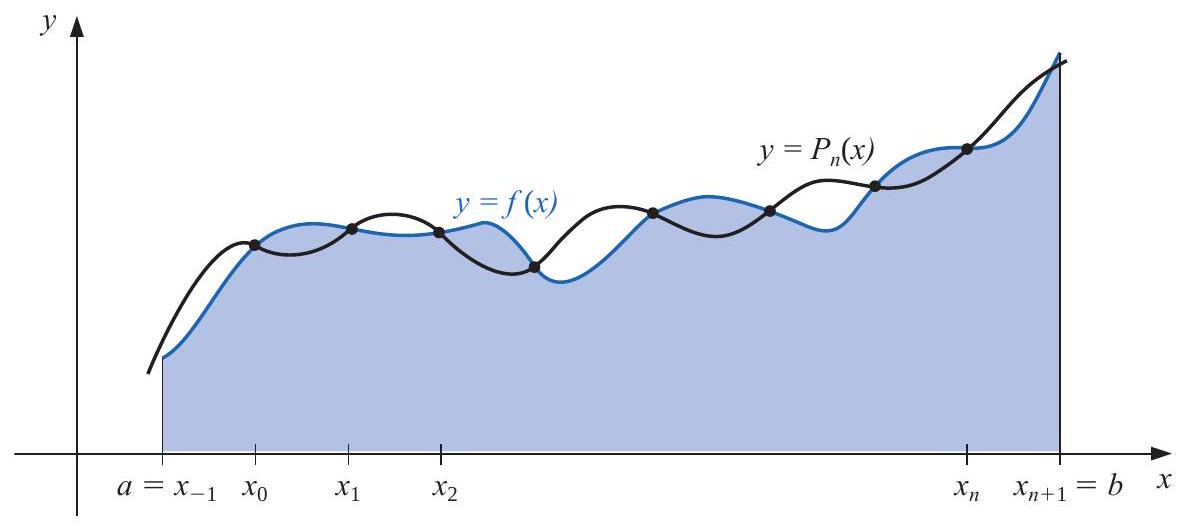
\includegraphics[width=12cm]{2025_05_15_85b7f7df47271a498e1dg-28}
\caption{\scriptsize Figure $10$}
\label{fig:opennewton1}
\end{figure}

The following theorem is analogous to Theorem \ref{thm:closednewtonecotes}

\begin{theorem}\label{thm:opennewtonecotes}
Suppose that $\sum_{i=0}^{n} a_{i} f\left(x_{i}\right)$ denotes the ( $n+1$ )-point open Newton-Cotes formula with $x_{-1}=a, x_{n+1}=b$, and $h=(b-a) /(n+2)$. There exists $\xi \in(a, b)$ for which

$$
\int_{a}^{b} f(x) d x=\sum_{i=0}^{n} a_{i} f\left(x_{i}\right)+\frac{h^{n+3} f^{(n+2)}(\xi)}{(n+2)!} \int_{-1}^{n+1} t^{2}(t-1) \cdots(t-n) d t
$$

if $n$ is even and $f \in C^{n+2}[a, b]$, and

$$
\int_{a}^{b} f(x) d x=\sum_{i=0}^{n} a_{i} f\left(x_{i}\right)+\frac{h^{n+2} f^{(n+1)}(\xi)}{(n+1)!} \int_{-1}^{n+1} t(t-1) \cdots(t-n) d t
$$

if $n$ is odd and $f \in C^{n+1}[a, b]$.
\end{theorem}

Notice, as in the case of the closed methods, we have the degree of precision comparatively higher for the even methods than for the odd methods.

Some of the common open Newton-Cotes formulas with their error terms are as follows:\\
{\bf $n=0$ : Midpoint rule}


\begin{equation}\label{eqn:opennewtoncotesmpnis0}
\int_{x_{-1}}^{x_{1}} f(x) d x=2 h f\left(x_{0}\right)+\frac{h^{3}}{3} f^{\prime \prime}(\xi), \quad \text { where } \quad x_{-1}<\xi<x_{1} 
\end{equation}


{\bf $n=1:$}


\begin{equation}\label{eqn:opennewtoncotesmpnis1}
\int_{x_{-1}}^{x_{2}} f(x) d x=\frac{3 h}{2}\left[f\left(x_{0}\right)+f\left(x_{1}\right)\right]+\frac{3 h^{3}}{4} f^{\prime \prime}(\xi), \quad \text { where } \quad x_{-1}<\xi<x_{2}
\end{equation}



{\bf $n=2:$}
\begin{equation}\label{eqn:opennewtoncotesmpnis2}
 \int_{x_{-1}}^{x_{3}} f(x) d x=\frac{4 h}{3}\left[2 f\left(x_{0}\right)-f\left(x_{1}\right)+2 f\left(x_{2}\right)\right]+\frac{14 h^{5}}{45} f^{(4)}(\xi) 
\end{equation}
 where  $ x_{-1}<\xi<x_{3}$.

{\bf $n=3$:}
\begin{equation}\label{eqn:opennewtoncotesmpnis3}
\int_{x_{-1}}^{x_{4}} f(x) d x=\frac{5 h}{24}\left[11 f\left(x_{0}\right)+f\left(x_{1}\right)+f\left(x_{2}\right)+11 f\left(x_{3}\right)\right]+\frac{95}{144} h^{5} f^{(4)}(\xi)
\end{equation}
where $x_{-1}<\xi<x_{4}$


\begin{example}
Compare the results of the closed and open Newton-Cotes formulas listed as \ref{eqn:closednewtontrap}-\ref{eqn:clsednewtonsimpsonnis4} and \ref{eqn:opennewtoncotesmpnis0}-\ref{eqn:opennewtoncotesmpnis3} when approximating

$$
\int_{0}^{\pi / 4} \sin x d x=1-\sqrt{2} / 2 \approx 0.29289322
$$
\end{example}

\begin{mysolution}
For the closed formulas we have

$$
\begin{aligned}
& n=1: \frac{(\pi / 4)}{2}\left[\sin 0+\sin \frac{\pi}{4}\right] \approx 0.27768018 \\
& n=2: \frac{(\pi / 8)}{3}\left[\sin 0+4 \sin \frac{\pi}{8}+\sin \frac{\pi}{4}\right] \approx 0.29293264 \\
& n=3: \frac{3(\pi / 12)}{8}\left[\sin 0+3 \sin \frac{\pi}{12}+3 \sin \frac{\pi}{6}+\sin \frac{\pi}{4}\right] \approx 0.29291070 \\
& n=4: \frac{2(\pi / 16)}{45}\left[7 \sin 0+32 \sin \frac{\pi}{16}+12 \sin \frac{\pi}{8}+32 \sin \frac{3 \pi}{16}+7 \sin \frac{\pi}{4}\right] \approx 0.29289318
\end{aligned}
$$

and for the open formulas we have

$$
\begin{array}{ll}
n=0: & 2(\pi / 8)\left[\sin \frac{\pi}{8}\right] \approx 0.30055887 \\
n=1: & \frac{3(\pi / 12)}{2}\left[\sin \frac{\pi}{12}+\sin \frac{\pi}{6}\right] \approx 0.29798754 \\
n=2: & \frac{4(\pi / 16)}{3}\left[2 \sin \frac{\pi}{16}-\sin \frac{\pi}{8}+2 \sin \frac{3 \pi}{16}\right] \approx 0.29285866 \\
n=3: & \frac{5(\pi / 20)}{24}\left[11 \sin \frac{\pi}{20}+\sin \frac{\pi}{10}+\sin \frac{3 \pi}{20}+11 \sin \frac{\pi}{5}\right] \approx 0.29286923
\end{array}
$$
\end{mysolution}
Table \ref{tab:intcomp} summarizes these results and shows the approximation errors.
%
%Table 4.8
%
\begin{table}[h]
\centering
\begin{tabular}{lccccc}
\hline
\multicolumn{1}{c}{$n$} & 0 & 1 & 2 & 3 & 4 \\
\hline
Closed formulas &  & 0.27768018 & 0.29293264 & 0.29291070 & 0.29289318 \\
Error &  & 0.01521303 & 0.00003942 & 0.00001748 & 0.00000004 \\
Open formulas & 0.30055887 & 0.29798754 & 0.29285866 & 0.29286923 &  \\
Error & 0.00766565 & 0.00509432 & 0.00003456 & 0.00002399 &  \\
\hline
\end{tabular}
\caption{\scriptsize Table 3: Comparison of Closed and Open Newton-Cotes Formulas}
\label{tab:intcomp}
\end{table}

\begin{myexercise}%\label{Comprehensionquiz2}
Consider the integral 
\[I=\int_1^{1.6}\frac{2x}{x^2-4}\,dx\]
\begin{enumerate}[label=(\alph*)]
\item Approximate the integral using the
\begin{enumerate}[label=\roman*.]
\item Trapezoidal rule
\item Simpson's rule
\item Midpoint rule
\end{enumerate}
\item Find abound for the error in each of the approximations in part (a) using the error formula, and compare this to the actual error.
\end{enumerate}

\begin{mysolution}
\begin{enumerate}[label=(\alph*)]
\item 
\begin{enumerate}[label=\roman*.]
\item $-0.8666667$
\item $-0.7391053$
\item $-0.6753247$
\end{enumerate}
\item 
\begin{enumerate}[label=\roman*.]
\item Actual error $=0.1326975$, Error bound $=0.5617284$
\item Actual error $= 5.1361\times10^{-3}$. Error bound $=0.063280$
\item Actual error $=0.0564448$, Error bound $=0.2808642$
\end{enumerate}
\end{enumerate}
\end{mysolution}
\end{myexercise}


%\discussion


\begin{posttest}%[\textcolor{red}{End of Module 4 Quiz}]
\item Construct and graph the cubic Bézier polynomials given the following points and guidepoints.
\begin{enumerate}[label=(\alph*)]
\item Point $(1,1)$ with guidepoint $(1.5,1.25)$ to point $(6,2)$ with guidepoint $(7,3)$\\
\item Point $(1,1)$ with guidepoint $(1.25,1.5)$ to point $(6,2)$ with guidepoint $(5,3)$\\
\item Point $(0,0)$ with guidepoint $(0.5,0.5)$ to point $(4,6)$ with entering guidepoint $(3.5,7)$ and exiting guidepoint $(4.5,5)$ to point $(6,1)$ with guidepoint $(7,2)$\\
\item Point $(0,0)$ with guidepoint $(0.5,0.5)$ to point $(2,1)$ with entering guidepoint $(3,1)$ and exiting guidepoint $(3,1)$ to point $(4,0)$ with entering guidepoint $(5,1)$ and exiting guidepoint $(3,-1)$ to point $(6,-1)$ with guidepoint $(6.5,-0.25)$ 
\end{enumerate}

\item Conside the data and the corresponding function that generated the data. Compute the actual errors, and find error bounds using the error formulas.

\begin{multicols}{2}
\begin{enumerate}[label=(\alph*)]
\item
\begin{center}
\begin{tabular}{c|c|l}
$x$ & $f(x)$ & $f^{\prime}(x)$ \\
\hline
0.5 & 0.4794 &  \\
0.6 & 0.5646 &  \\
0.7 & 0.6442 &  \\
\end{tabular}
\end{center}

\[f(x)=\sin x\]
\item
\begin{center}
\begin{tabular}{c|l|l}
$x$ & \multicolumn{1}{|c|}{$f(x)$} & $f^{\prime}(x)$ \\
\hline
0.0 & 0.00000 &  \\
0.2 & 0.74140 &  \\
0.4 & 1.3718 &  \\
\end{tabular}
\end{center}

 \[f(x)=e^{x}-2 x^{2}+3 x-1\]
\end{enumerate}
\end{multicols}

\item Apply the extrapolation process described in Example \ref{Richardsonsexample1} to determine $N_{3}(h)$, an approximation to $f^{\prime}\left(x_{0}\right)$, using four-digit rounding arithmetic for the following functions and stepsizes.
%%\begin{multicols}{2}
\begin{enumerate}[label=(\alph*)]
\item $\quad f(x)=\ln x, x_{0}=1.0, h=0.4$\\
\item $\quad f(x)=x+e^{x}, x_{0}=0.0, h=0.4$\\
\item $\quad f(x)=2^{x} \sin x, x_{0}=1.05, h=0.4$\\
\item $\quad f(x)=x^{3} \cos x, x_{0}=2.3, h=0.4$
\end{enumerate}
%\end{multicols}
\item Consider the integral 
\[I=\int_0^{\pi/4}e^{3x}\sin2x\,dx\]
\begin{enumerate}[label=(\alph*)]
\item Approximate the integral using the
\begin{enumerate}[label=\roman*.]
\item Trapezoidal rule
\item Simpson's rule
\item Midpoint rule
\end{enumerate}
\item Find abound for the error in each of the approximations in part (a) using the error formula, and compare this to the actual error.
\end{enumerate}

\begin{mysolution}
\begin{enumerate}[label=\arabic*.]
\item
\begin{enumerate}[label=(\alph*)]
\item $x(t)=-11.5t^3+15t^2+1.5t+1$, $y(t)=-4.25t^3+4.5t^2+0.75t+1$
\item $x(t)=-6.25t^3+10.5t^2+0.75t+1$, $y(t)=-3.5t^3+3t^2+1.5t+1$
\item For $t$ between $(0,0)$ and $(4,6)$, we have
\[x(t) =-5t^3 +7.5t^2 +1.5t,\quad y(t) =-13.5t^3 +18t^2 +1.5t,\]
and for $t$ between $(4,6)$ and $(6,1)$, we have
\[x(t) =-5.5t^3 + 6t^2 +1.5t +4,\quad y(t) = 4t^3 -6t^2-3t +6.\]
\item For t between $(0,0)$ and $(2,1)$, we have
\[x(t) =-5.5t^3 + 6t^2 +1.5t,\quad y(t) =-0.5t^3 +1.5t,\]
for $t$ between $(2,1)$ and $(4,0)$, we have
\[x(t) =-4t^3 +3t^2 +3t +2,\quad y(t) =-t^3 +1,\]
and for $t$ between $(4,0)$ and $(6,-1)$, we have
\[x(t) =-8.5t^3 + 13.5t^2-3t +4,\quad y(t) =-3.25t^3 +5.25t^2-3t.\]
\end{enumerate}
\item
\begin{center}
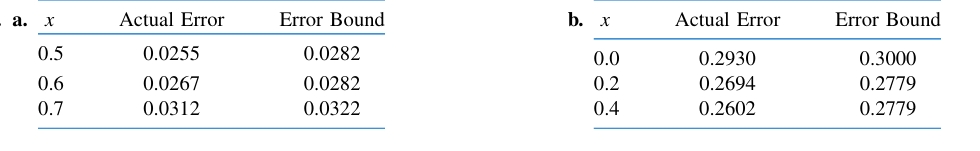
\includegraphics[width=15cm]{EndofMod4Q2sol}
\end{center}
\item
\begin{multicols}{2}
\begin{enumerate}[label=(\alph*)]
\item $f(1)\approx1.001$ \item $f(0)\approx1.999$ \item $f(1.05)\approx2.283$ \item $f(2.3)\approx-19.61$
\end{enumerate}
\end{multicols}
\item 
\begin{enumerate}[label=(\alph*)]
\item 
\begin{enumerate}[label=\roman*.]
\item $4.1432597$
\item $2.5836964$
\item $1.8039148$
\end{enumerate}
\item 
\begin{enumerate}[label=\roman*.]
\item Actual error $=1.554631$, Error bound $=2.298827$
\item Actual error $= 4.9322\times10^{-3}$. Error bound $=0.1302826$
\item Actual error $=0.7847138$, Error bound $=1.1494136$
\end{enumerate}
\end{enumerate}
\end{enumerate}
\end{mysolution}
\end{posttest}

%share your understanding of properties of functions and their applications to solving rates of change problems in physical phenomenon 


%\end{actsoln}

\takehome

\comy{You are now at the last part of this module. Your  task is to do a self-reflection on your learning experience.}



\references
\begin{refenumerate}
\item Kong, Q., Siauw, T., Bayen, A., (2020). Python Programming and Numerical Methods. First Edition, Academic Press,  ISBN-13 ‏ : ‎ 978-0128195499 \\
%chapter 1 pg 7-36 functions\\
%chapter 1 pg 51-83 limits and continuity\\
%chapter 1 pg 45-50 rates of change\\
%chapter 2 pg 108-120 the derivative\\
%\item Mendelson, E. (2022). Schaum's Outline of Calculus. McGraw-Hill Education.
%chapter 6 51-55 functions
%chapter 7 59-65 limits
%chapter 8 69-74 continuity
%chapter 9 77-81 derivative
%\item Calculus \mylink{https://math.libretexts.org/Bookshelves/Calculus}
%\item Chris McMullen, 2021, Essential Calculus Skills Practice Workbook with Full Solutions, Zishka Publishing, ISBN 978-1-941691-24-3
%\item R. Adams and C. Essex, 2021, Calculus: A complete Course, Addison Wesley, ISBN 13: 978-0135732588
%\item P. Abbott and H. Neill, 2018, Calculus: A Complete Introduction: The Easy Way to Learn Calculus (Teach Yourself), ISBN 13: 978-1473678446
\end{refenumerate}





%\wrapup
%To wrap-up, answer the following questions:
%
%\begin{enumerate}
%\item 
%%when do we say that a limit of a function exists?
%%\item how do we remove discontinuity in functions?
%%\item what is the relationship between the gradient of the tangent line and the derivative?
%\end{enumerate}
















%\newpage

%\facilitation


%
\begin{center}
    {\Large \textbf{FUNCTIONS OF SEVERAL VARIABLES}}\\[2mm]
(DEFINITION, DOMAIN, RANGE, GRAPHS AND LEVEL CURVES) \\[4mm]

\mycenterbox{5 minute review}%\\[4mm]
Recap the definition of a function of several variables, and the meaning of domain, range, graph and level curves of functions of several variables.
\end{center}
\mycenterbox{Warm-up.}%\\[4mm]
\problemAnswer{
Match the function with its graph (labeled I–VI).Give reasons for your choices
\begin{multicols}{3}
\begin{enumerate}[label=(\alph*)]
\item $f(x,y)=|x|+|y|$\\[4mm]
\item $f(x,y)=|xy|$
\item $f(x,y)=\frac{1}{1+x^2+y^2}$\\2mm]
\item $f(x,y)=(x^2-y^2)^2$
\item $f(x,y)=(x-y)^2$\\[4mm]
\item $f(x,y)=\sin(|x|+|y|)$
\end{enumerate}
\end{multicols}

\begin{center}
%\centering
\includegraphics[width=10cm]{MCTutorial1Q1.JPEG}
\end{center}
%\tcbox[tcbox raise base]{Warm-up}
 
%\begin{flushright}
%\begin{tikzpicture}
%    % A body
%
%
%    % Non-rectangle shapes must be drawn as polygone
%    \begin{scope}[shift={(3,0)}]
%        \draw  (0,0.5) -- (0,4) -- (.5,4) -- (.5,4.5) -- (1.,4.5) -- (4.,4.5) --(4.,4)-- (4.5,4) --(4.5,0.5) --(4.0,0.5)--(4.0,0.0)-- (.5,0) --(0.5,0.5) -- cycle;
%        % Draw symmetry lines
%        \draw [symmetry] (.5, 0.5) -- (.5,4.0);
%        \draw [symmetry] (4, 0.5) -- (4,4.0);
%        \draw [symmetry] (.5,4.0) -- (4,4.0);
%         \draw [symmetry] (.5, 0.5) -- (4, 0.5);
%        % Dimensions
%        \draw (4.5,0) -- ++(0.5,0) coordinate (D1) -- +(5pt,0);
%        \draw (4.5,4.5) -- ++(0.5,0) coordinate (D2) -- +(5pt,0);
%        \draw [dimen] (D1) -- (D2) node {6cm};
%       
%        
%        \draw (0.0,5) -- ++(0,0.5) coordinate (D1) -- +(0,+5pt);
%        \draw (0.5,5) -- ++(0,0.5) coordinate (D2) -- +(0,+5pt);
%        \draw [dimen,-] (D1) -- (D2) node [above=5pt] {$x$ cm};
%        \draw [dimen,<-] (D1) -- ++(-5pt,0);
%        \draw [dimen,<-] (D2) -- ++(+5pt,0);
%    \end{scope}
%\end{tikzpicture}
%\end{flushright}

}


\mycenterbox{Problems.}%

%\begin{center}
%\tcbox[tcbox raise base]{ Problems. Choose from the below}
%\end{center}
\problem{Exploring functions}%
\begin{enumerate}[(a)]
\item Are the following functions even, odd, or neither? What can you say
about their range?
\begin{multicols}{4}
 \begin{enumerate}[(i)]
\item $\displaystyle \frac{3x}{x^2+2}$
\item $\displaystyle \cos x+3$
\item $\displaystyle \frac{2x^3}{\cos x+3}$
\item $\displaystyle \frac{3x^4+2x^2}{\sin x+4}$
\end{enumerate}
\end{multicols}
\item Consider the functions $\sin^n x$ and $\cos^n x$, where $n$ is a positive integer.
Which are odd, which are even, and what are their periodicities?
\item What is the periodicity of $f(x) = 2 \cos x+\sin 2x$? Is it even/odd/neither?

\end{enumerate}

\problem{Cubic functions} 
Show that $x-1$ is a factor of the cubic function%
$$P(x)=x^3-2x^2-5x+6,$$
and  find the quadratic factor $Q(x)$ such that $P(x) = (x -1)Q(x)$. Factorise
$Q(x)$ and hence sketch $P(x).$

%\newpage
\problem{Sigmoid functions*.}%
For positive integers $n$, consider the family of functions
$$\displaystyle f_n= \frac{x^n}{2^n+x^n}.$$
\begin{enumerate}[(a)]
\item What are appropriate domains and ranges for $f_n(x)$? Do they depend on $n$?

\item Is $f_n(x)$ even, odd, or neither? Does this depend on $n$?

\item Show that for $x\geq 0$, $f_n(x)$ are strictly increasing functions and that
$0\leq f_n(x) < 1.$
\item What is the value of $f_n(2)$? Does it depend on $n$?

\item By considering the values of $f_n(1.9)$ and $f_n(2.1)$ for $n = 2, 4, 8, 16, 32$ and
$64$, show that the graph of $f_n(x)$ for $x\ge 0$ is an increasing sigmoid (that
is, $S$-shaped) function that approaches a step function as $n\rightarrow \infty$.
\end{enumerate}

\mycenterbox{Selected answers and hints}%

For the warm-up, $V(x)=4x(3-x)^2$. Writing $x=1+\epsilon$, we get
$$V = 4(1 +\epsilon)(3- (1+\epsilon))^2=4(4-\epsilon^2(3-\epsilon)).$$
If $-1<\epsilon<2$ then $\epsilon^2 (3-\epsilon)\ge 0$, with equality when $\epsilon=0$. Thus the maximum
value of $V$ occurs when $\epsilon= 0$, i.e. $x = 1\rm{cm}$.

\begin{enumerate}
\item 
\begin{enumerate}[(i)]
\item Odd. The range is the interval  $[-\frac{3}{4}\sqrt{2},\; \frac{3}{4}\sqrt{2}]$
\item Even. The range is the interval $[2, 4]$.
\item Odd. The range is all of $\mathbb R$.
\item Neither. (For example, writing $\displaystyle \frac{5}{\sin x+4}$ we have $\displaystyle f(1)= \frac{5}{\sin (1)+4} \equiv 1.032 (3\rm{dp})$ which is neither $f(1)$ nor $-f(1)$.)\\[4mm]
The range is the nonnegative reals $[0,\infty)$

\end{enumerate}
\end{enumerate}










